

%====================================================================
\section{Introduction}
\label{sec:intro}
With the prevalence of data in various domains, experts including biologists start to engage in making sense of the data, mining knowledge and finding insight from the data. 
More and more biologists turn to data mining and machine learning toolkits for data analysis. However, before digging into these time-consuming data mining algorithms, there is usually a data exploration step, helping data scientists have a better overview of the data and forming hypothesis for further analysis. In this paper, we propose a toolkit, titled as \genviz, and envision it as a data exploration toolkit for {\em separability} analysis. Separability, a common problem in biology, is defined as: given two different classes of objects and a feature-object matrix, find the best k features (\topk) separating these two classes. Many biological applications fit in this framework. For instance, when cells are exposed to a drug treatment, a set of genes may be differentially expressed while the other genes are not. Given the result for such a drug treatment experiment, biologists often want to find features to characterize these differentially expressed genes. \silu{FIX the example?}
In \genviz, we focus on finding \topk feature pairs instead of more commonly identified \topk single features. This is because 
{\em (a)} a single feature can be considered as a special case of a feature pair by taking the same feature in a feature pair;
{\em (b)} a combined feature pair is likely to provide new insight compared to single features;
{\em (c)} feature pair can be easily visualized in a 2-D space.
As we will illustrate in Section~\ref{sec:exp}, two features that rank poorly on their own may have very good separability when combined together. We will carefully describe the problem formulation later in Section~\ref{sec:method}. 

%Information Visualization

There are three key aspects in \genviz. First, there is the interesting challenge of given a feature pair, how to measure its quality in separating different classes of objects. Second, how to quickly identify \topk feature pairs based on a separability metric is also a big concern since small latencies are critical for a data exploration tool like \genviz. Last but not least, the output of \genviz is not just the \topk feature pairs, but also the corresponding visualizations. The output visualizations can help the users better interpret the result, i.e., how different classes of objects are separated from each other. In the following, we elaborate more on these three points. 



\stitle{Separability Metric.} Many existing separability metrics focus on identifying relevant single features instead of feature pairs. For instance, in order to characterize differentially expressed genes (DEG), biologists typically do association test (e.g, hypergeometric test) to find the best single feature that enriches in the DEG set compared to the other genes \silu{FIX this example?}. However, we demonstrate in Section~\ref{sec:exp} that feature pairs can provide additional insights that are not revealed by top single features. Hence, developing a meaningful separability metric for feature pairs is the first and an important step towards developing separability analysis method. Furthermore, since \genviz has visualizations as the intended primary output instead of a pure separability score, our proposed separability metric should encode visual separability to some extent. 

\stitle{Fast Identification.} Since \genviz serves as a data exploration tool before applying more sophisticated machine learning algorithms, we prioritize optimizing its running time over its accuracy. In some sense, we designed \genviz as a  {\em "quick and dirty"} way to solve the separability problem. Thus, instead of more-complex machine learning methods, we prefer light-weight separability metrics combined with various optimization mechanisms to reduce running time. 

\stitle{Visualization Output.} Given a separating feature pair, it is natural to visualize the object sets in a two dimensional space where the x-axis and y-axis represent two single features respectively. Thus, there is a one-to-one relationship between a visualization and a feature pair, which allows the users to  easily gain  a general sense of how different classes of objects are separated for a given feature pair. Looking at the visualization leads to a better understanding of the results compared to the pure separability score.




%\newpage
%==================================================================
\section{Method}
\label{sec:method}
In Section~\ref{sec:intro}, we argued the motivation for \genviz. In this section, we begin with the formal definition of the {\em separability} problem, then introduce the proposed separability metric, and finally develop various optimization algorithms for fast identification.
\subsection{Problem Definition}\label{sec:prob}
%In Section~\ref{sec:intro}, we have talked about different biology applications that can be abstracted as a separability problem. In this section, we will formally formulate the problem and discuss the challenges in it. 

\begin{table}[t!]
\centering
\small
\begin{tabular}{c|c|c|c}
  %\hline
   Symb. & Description & Symb. & Description\\
    \hline
    \hline
    $\mm$ & feature-object matrix & $\ff$ & feature set in $\mm$ \\
    \hline
    $f_i$ & feature $i$ in $\ff$ & $m$ & number of features in $\ff$\\
    \hline
    $\oo$ & object set in $\mm$ & $N$ & number of objects in $\oo$\\
    \hline
    $\oo_+$ & positive object set & $\oo_-$ & negative object set\\
    \hline
    $\widehat{\oo}$ & labelled object set & $n$ & number of labelled objects in $\widehat{\oo}$\\
    \hline
    $o_k$ & object $k$ in $\widehat{\oo}$ & $l_k$ & label of object $o_k$\\
    \hline
    $\ell$ & separating line in 2-D & $\hat{\ell}$ & representative line  in 2-D\\
    \hline
    $\eta_{i,j}^{\ell,k}$ & predicted label of $o_k$ & $\theta_{i,j}^{\ell,k}$ & $o_k$ is correctly separated? \\
    \hline
    $\theta_{i,j}^{\ell}$ & \# correctly separated $o_k$ & $\theta_{i,j}$ & separability score\\
    \hline
    $\widehat{\mm}$ & $\mm$ after transformation &  $\tilde{\theta}_{i,j}$ & estimated $\theta_{i,j}$\\
    \hline
 \end{tabular}
\caption{Notations}
\label{tbl:notation}
\vspace{-18pt}
\end{table}

\begin{figure*}[t]
  \centering
  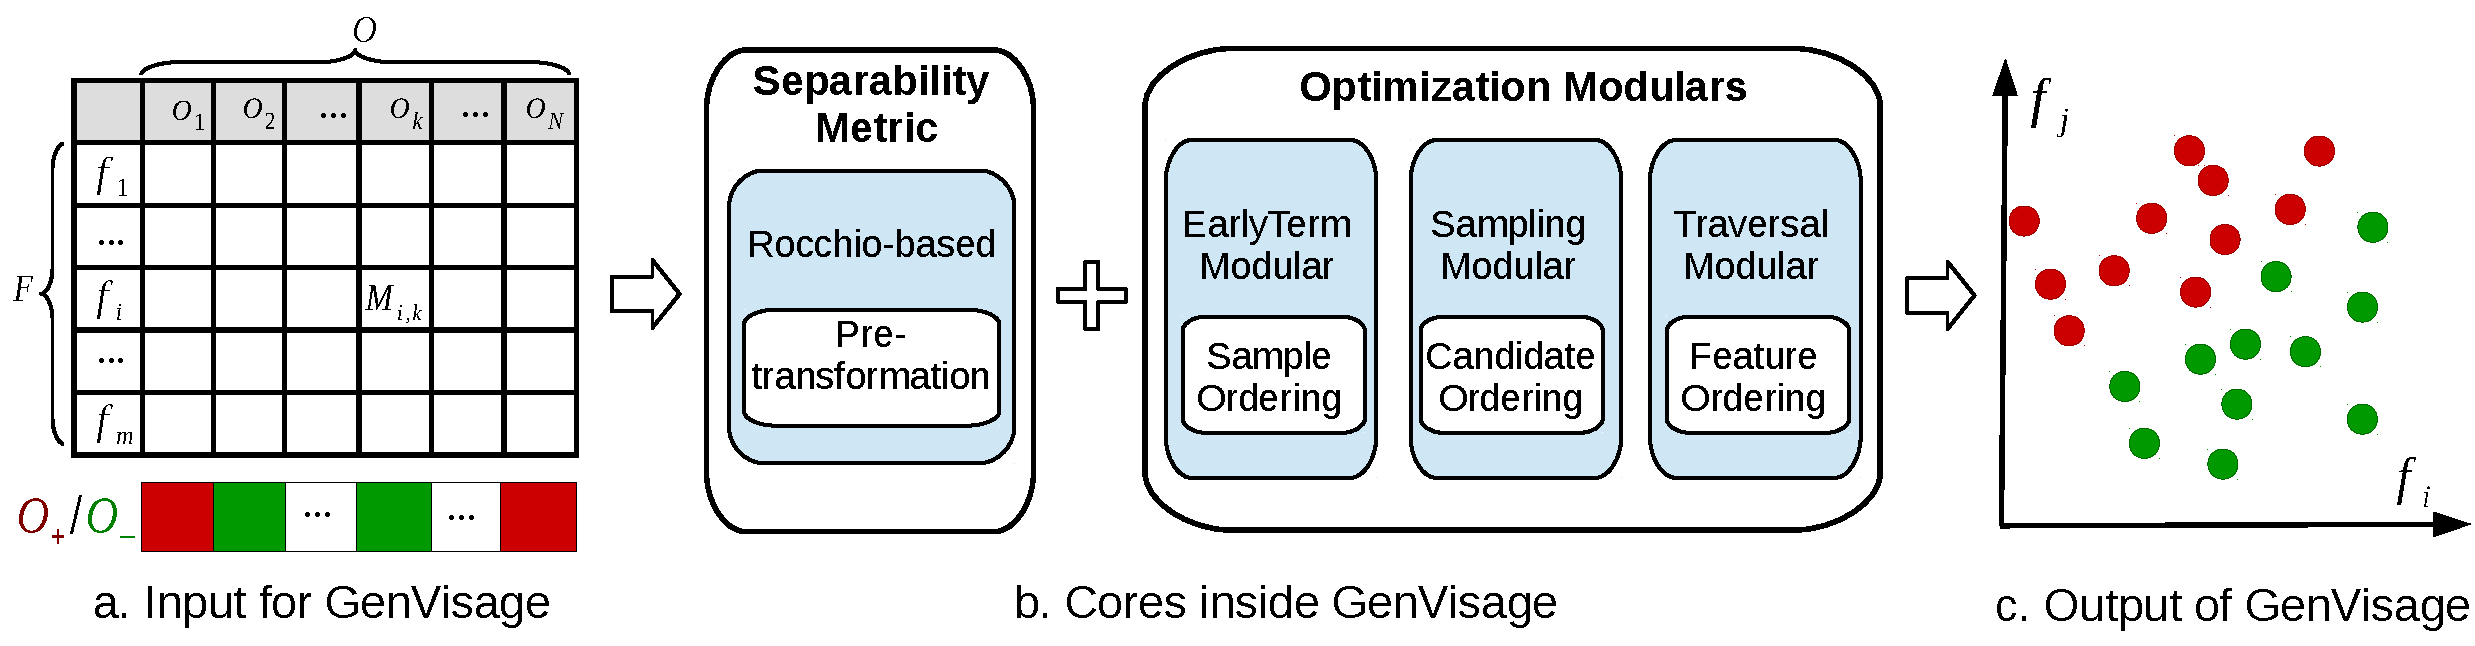
\includegraphics[width=0.9\linewidth]{fig/workflow2.pdf}
\caption{\genviz Workflow}
\label{fig:workflow}
\end{figure*} 


We first introduce some essential notations. Let $\mm$ be a feature-object matrix of size $m\times N$, where each row is a feature and each column is an object. Correspondingly, denote the $m$ features as $\ff=\{f_1,f_2,\cdots,f_m\}$ and $N$ objects as $\oo=\{o_1,o_2,\cdots,o_N\}$. Each entry $\mm_{i,j}$ in $\mm$ is of numeric type, representing the value of object $o_j$ on feature $f_i$. In addition, we are given two non-overlapping sets of objects, one with positive label and the other with negative label, denoted as $\oo_+$ and $\oo_-$ respectively. Both sets of positive and negative objects are subsets of all objects, i.e., $\oo_+\subset \oo$ and $\oo_-\subset \oo$. Let $\widehat{\oo}$ be the union of both positive and negative objects and $n$ be the total number of labelled objects, i.e., $\widehat{\oo}=\oo_+\cup \oo_-$, $n=|\widehat{\oo}|$ and $n\leq N$. Accordingly, let $l_k$ be the label of object $o_k\in \widehat{\oo}$, i.e., $l_k=1$ if $o_k$ is positive and $l_k=-1$ if $o_k$ is negative. 

Now we are ready to formally describe the task of \genviz. The overall workflow is depicted in Figure~\ref{fig:workflow}: given a matrix $\mm$ and two object sets $\oo_+$ and $\oo_-$, \genviz aims to find feature pairs to separate $\oo_+$ from $\oo_-$, and output a visualization to explain the separability. Furthermore, since we are targeting as a data exploration tool before more time-consuming machine learning methods, our design principle allows for small sacrifices to accuracy for great improvements in running time. We formally define the separability problem in Problem~\ref{prob:separability}. 

%discriminative 

% \begin{figure}[h]
%   \centering
%   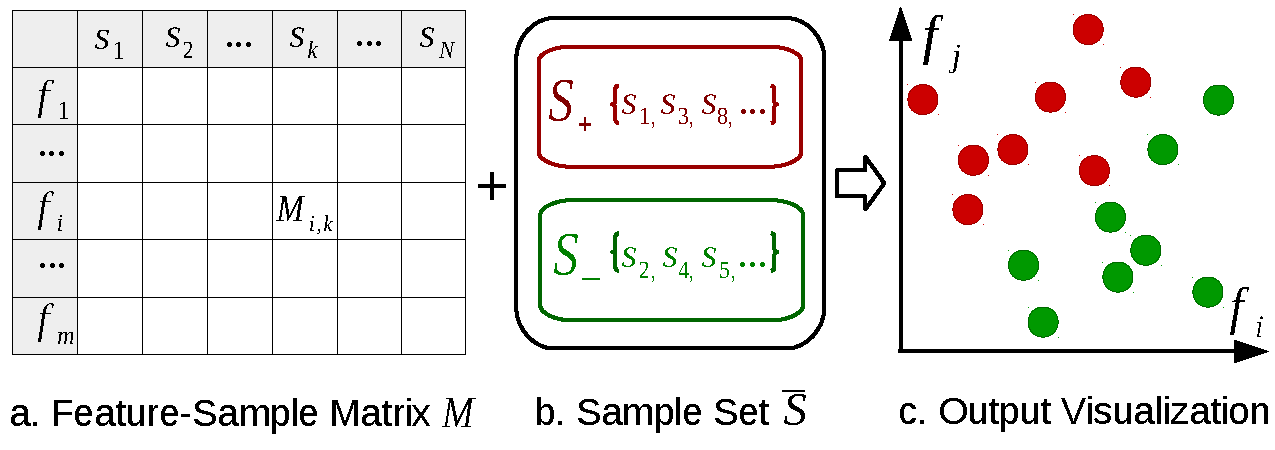
\includegraphics[width=\linewidth]{fig/workflow.pdf}
% \caption{\genviz Workflow}
% \label{fig:workflow}
% \end{figure} 


% \slhuang{feature pair is }
\begin{formulation}[Separability]\label{prob:separability}
Given a feature-object matrix $\mm$ and two labeled object sets $(\oo_+,\oo_-)$, \textbf{fast identify} \topk feature pairs $(f_i,f_j)$ separating $\oo_+$ from $\oo_-$ based on a given \textbf{separability metric}, and output a 2-D {visualization}.
\end{formulation}


As highlighted in Problem~\ref{prob:separability}, how to define a separability metric and how to fast identify \topk feature pairs pose great challenges in \genviz. In the following, we will first describe our selected separability metric in Section~\ref{sec:metric}, and then discuss different optimization techniques in Section~\ref{sec:opt}.



%==================================================================
\subsection{Separability Metric}\label{sec:metric}
Given a feature pair $(f_i,f_j)$, we can visualize $\oo_+$ and $\oo_-$ in a 2-D space. Since linear separability is more intuitive and explainable visually, in this paper we focus on linear separability~\cite{shamos1975geometric} and propose linear separability metric for a given 2-D visualization. 

Let us first review the concept of {\em linear separability} introduced in Euclidean geometry~\cite{shamos1975geometric}. The sets of objects, i.e., $\oo_+$ and $\oo_-$, are \emph{linearly separable} if there exists at least one straight line in the plane such that all points from $\oo_+$ are on one side of the line, while all points from $\oo_-$ are on the other side of the line. Mathmatically, we can represent a line $\ell$ using Equation~\ref{eqn:line}, where $x$ and $y$ represent an object's value on feature $f_i$ and $f_j$ respectively, and $w_0$, $w_i$ and $w_j$ are coefficients. Given a feature pair $(f_i,f_j)$ and a line $\ell$, let $\eta_{i,j}^{\ell,k}$ be the predicted label of an object $o_k$. The predicted label $\eta_{i,j}^{\ell,k}$ is calculated according to Equation~\ref{eqn:est_label}: if $o_k$ lies above the line $\ell$, then $\eta_{i,j}^{\ell,k}=1$; otherwise, $\eta_{i,j}^{\ell,k}=-1$.   
If there exists a line $\ell$ such that for any objects $o_k\in \widehat{\oo}$, the predicted label $\eta_{i,j}^{\ell,k}$ is consistent with the real label $l_k$, i.e., $\eta_{i,j}^{\ell,k}\cdot l_k = 1$, then we say $\oo_+$ and $\oo_-$ are linear separable. 
%as shown in Equation~\ref{eqn:linear}
\begin{equation}\label{eqn:line}
\begin{split}
\ell: \hspace{4mm} w_i\cdot x + w_j\cdot y +w_0 =0 
\end{split}
\end{equation}
\begin{equation}\label{eqn:est_label}
{\sf Predicted \hspace{1mm} Label:}\hspace{3mm} \eta_{i,j}^{\ell,k}=sign(w_i\cdot \mm_{i,k} + w_j\cdot \mm_{j,k} +w_0)
\end{equation}
% \begin{equation}\label{eqn:linear}
% \eta_{i,j}^{\ell,k} = \left\{
%                 \begin{array}{ll}
%                   1 \textit{\hspace{2mm} if \hspace{2mm}} o_k\in \oo_+, \textit{ i.e., } l_k=1 \\
%                   -1 \textit{\hspace{2mm} if \hspace{2mm}} o_k\in \oo_-, \textit{ i.e., } l_k=-1 
%                 \end{array}
%               \right.
% \end{equation}

%%\sign
\vspace{2mm} %We stress on visual explainability, and linear separability in a 2-D visualization can be easily recognized and interpreted by the users. %, i.e., $\eta_{i,j}^{\ell,k}\cdot l_k = 1$, 
Next, let us introduce our proposed separability metric. Our proposed separability metric is based on linear separability and is defined as {\em how well a 2-D visualization can be linearly separated}. Let us formally define the separability metric.
First, given a feature pair $(f_i, f_j)$ and a line $\ell$, let $\theta_{i,j}^{\ell,k}$ be the variable indicating whether an object $o_k$ is correctly separated, as depicted in Equation~\ref{eqn:s_object}.
Then, given a feature pair $(f_i, f_j)$ and a line $\ell$, the separability score is defined as the number of correctly separated objects, denoted as $\theta_{i, j}^\ell$ as shown in Equation~\ref{eqn:s_line}. Figure~\ref{fig:brute_force} shows different separability scores $\theta_{i, j}^\ell$ with different separating lines. Finally, the separability score for a feature pair $(f_i,f_j)$ is defined as the best $\theta_{i, j}^{\ell}$ among all possible lines $\ell$, denoted as $\theta_{i, j}$ as shown in Equation~\ref{eqn:s_viz}. 
\begin{equation}\label{eqn:s_object}
\theta_{i,j}^{\ell,k}=\left\{
                \begin{array}{ll}
                  1 \textit{\hspace{2mm} if \hspace{2mm}} \eta_{i,j}^{\ell,k}\cdot l_k = 1\\
                  0 \textit{\hspace{2mm} otherwise \hspace{2mm}} 
                \end{array}
              \right.
\end{equation}
\begin{equation}\label{eqn:s_line} 
\hspace{3mm} \theta_{i,j}^{\ell}= \sum_{k}{\theta_{i,j}^{\ell,k}} %{\sf Separability \hspace{1mm} Score\hspace{1mm} with\hspace{1mm} Line\hspace{1mm} \ell:}
\end{equation}
\begin{equation}\label{eqn:s_viz}
\hspace{3mm} \theta_{i,j}= \max_{\ell}\{\theta_{i,j}^{\ell}\} %{\sf Separability \hspace{1mm} Score:}
\end{equation}

%The basic intuition is that the users can easily recognize and interpret linear separability in a 2-D visualization. Thus if a visualization is perfectly linearly separated, it should have high score in our proposed separability metric; otherwise, we would find the best separating line $\ell$ in the visualization and report the largest number of correctly separated objects as the separability score.\silu{talk about weighted case}


%%%%%%%%%%%%%%%%%%%%%%%%%%%%%%%%%%NEED TOGGLE%%%%%%%%%%%%%%%%%%%%%%
% \begin{figure}[h]
%   \centering
%   \begin{subfigure}{0.235\textwidth}
%     \centering
%     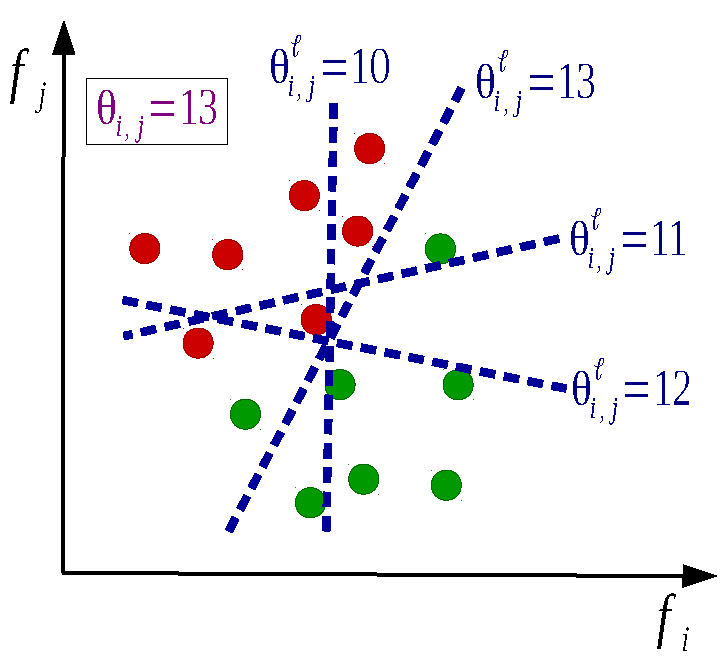
\includegraphics[width=\linewidth]{fig/metric.pdf}
%     \vspace{-5mm}
%     \caption{Brute Force}%{$\theta_{i,j}^{\ell}$ with Different Lines}
%     \label{fig:brute_force}
%   \end{subfigure}
%   \begin{subfigure}{.235\textwidth}
%     \centering
%     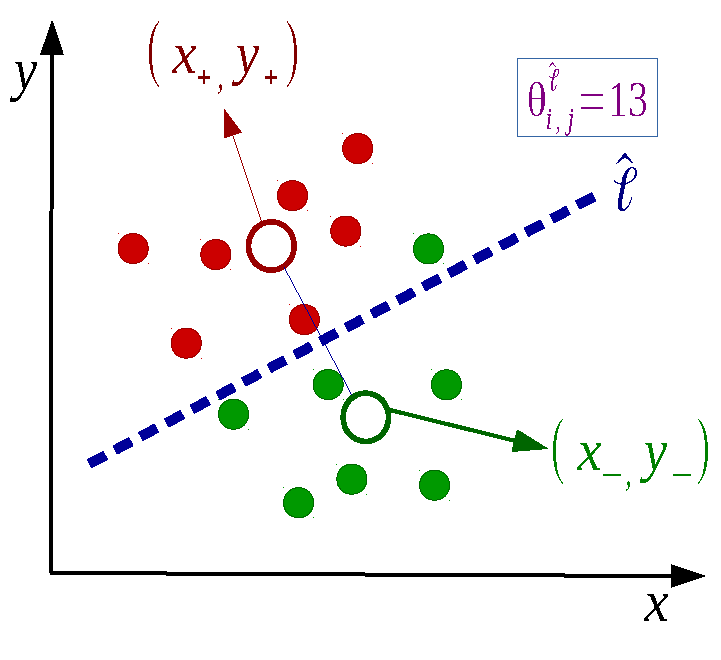
\includegraphics[width=\linewidth]{fig/rocchio.pdf}
%     \vspace{-5mm}
%     \caption{Rocchio-Based}%{$\theta_{i,j}^{\hat{\ell}}$ with Representative Line}
%     \label{fig:rocchio}
%   \end{subfigure}
% \caption{Different methods to Calculate Separability Score $\theta_{i,j}$}
% \label{fig:metric}
% \end{figure} 

\begin{figure}[h]
\centering     %%% not \center
\vspace{-5mm}
\subfigure[Brute Force]{\label{fig:brute_force}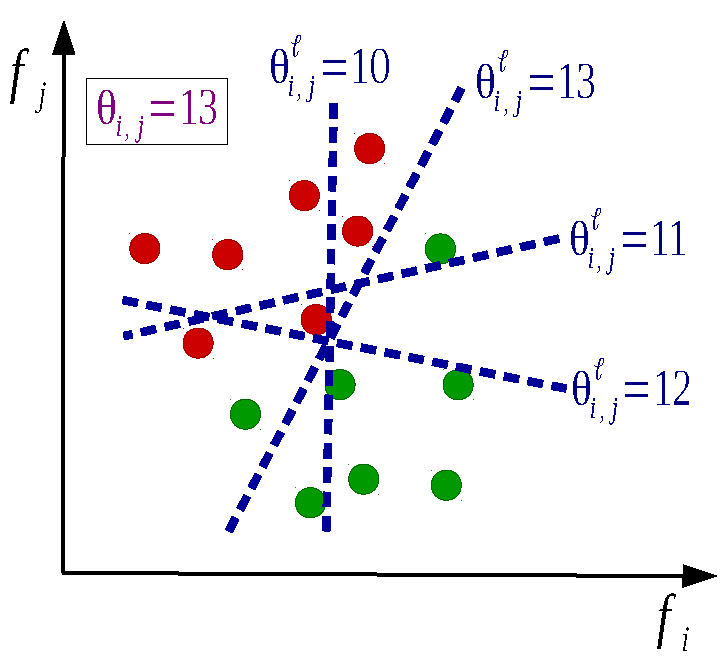
\includegraphics[width=.235\textwidth]{fig/metric.pdf}}
\subfigure[Rocchio-Based]{\label{fig:rocchio}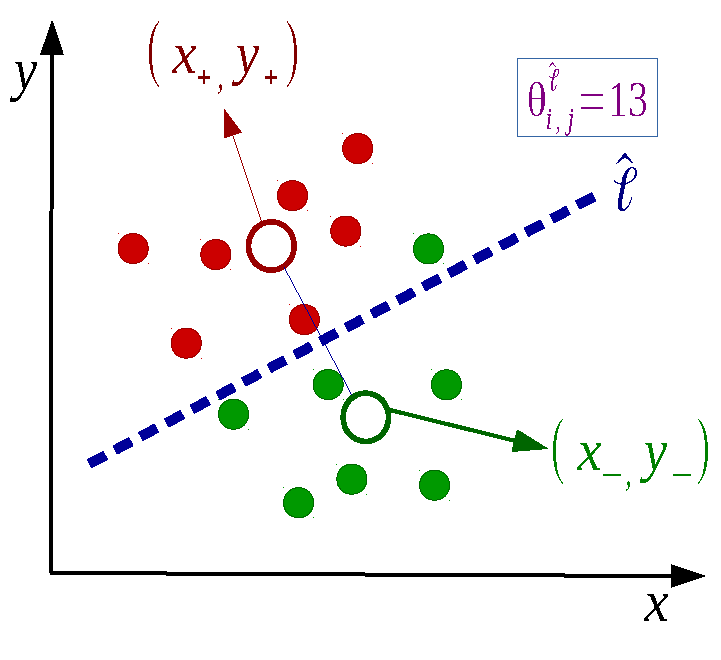
\includegraphics[width=.235\textwidth]{fig/rocchio.pdf}}
\vspace{-5mm}
\caption{Different Methods to Calculate Separability Score $\theta_{i,j}$}
\vspace{-5mm}
\label{fig:metric}
\end{figure}


\stitle{Brute Force.} As suggested in Figure~\ref{fig:brute_force}, the brute force way to calculate $\theta_{i,j}$ is to first enumerate all possible separating lines $\ell$ and calculate each $\theta_{i,j}^\ell$. This is infeasible as there are infinite number of possible lines. However, we can easily trim down the search space to $O(n^2)$ lines by linking the points for every two objects in the 2-D plane. This is because the results of all other possible lines can be covered by these $O(n^2)$ lines. Nevertheless, it is still very time-consuming to consider $O(n^2)$ lines for each feature pair $(f_i,f_j)$. 

\stitle{Rocchio-based.} We propose to use a {\em representative line} $\hat{\ell}$ to approximate $\theta_{i, j}$ as shown in Equation~\ref{eqn:s_viz_appr}, rather than considering all $O(n^2)$ possible lines and finding the one that satisfies Equation~\ref{eqn:s_viz}. 
\begin{equation}\label{eqn:s_viz_appr}
\theta_{i,j}  \approx \theta_{i,j}^{\hat{\ell}}
\end{equation}
Now, the search space is reduced to $O(1)$ from $O(n^2)$. The representative line is seleced based on Rocchio's algorithm~\cite{rocchio1971relevance}. 
%As we will show later in Section~\ref{sec:exp}, $\theta_{i,j}^{\hat{\ell}}$ is comparable to $\theta_{i,j}$ when using Rocchio-based representative line $\hat{\ell}$. Let us describe in detail about the Rocchio-based representative line.
The intuition behind Rocchio's algorithm is that each object's label should be consistent with its nearest centroid. Thus, we predict each object's label the same as its nearest centroid. More specifically, let us denote the centroids of positive objects $\oo_+$ and negative objects $\oo_-$ for a given $(f_i,f_j)$ as $\mu_+=(\mm_i^+,\mm_j^+)$ and $\mu_-=(\mm_i^-,\mm_j^-)$ respectively. The perpendicular bisector of the two centroids is selected as the representative separating line $\hat{\ell}$. Mathematically, $\hat{\ell}$ can be represented using Equation~\ref{eqn:line} with instantiated $w_i$, $w_j$ and $w_0$ as shown in Equation~\ref{eqn:rep_line}. Figure~\ref{fig:rocchio} illustrates the centroids $\mu_+$ and $\mu_-$, as well as the Rocchio-based representative separating line $\hat{\ell}$. In the figure, the estimated $\theta_{i,j}^{\hat{\ell}}$ equals $13$ with one negative object (green point in Figure~\ref{fig:rocchio}) mis-predicted as positive, while the real $\theta_{i,j}$ also equals $13$.




%\hat{\ell}: \hspace{4mm} (\mm_i^+-\mm_i^-)\cdot x + (\mm_j^+-\mm_j^-)\cdot y -(\frac{(\mm_i^+)^2-(\mm_i^-)^2}{2}+\frac{(\mm_j^+)^2-(\mm_j^-)^2}{2}) =0 

\begin{equation}\label{eqn:rep_line}
\begin{split}
& w_i = \mm_i^+-\mm_i^- \\
& w_j = \mm_j^+-\mm_j^- \\
& w_0 = -(\frac{(\mm_i^+)^2-(\mm_i^-)^2}{2}+\frac{(\mm_j^+)^2-(\mm_j^-)^2}{2})
\end{split}
\end{equation}


\stitle{Brute-force vs. Rocchio-based.} Compared to brute force, Rocchio-based method is much more light-weight in terms of running time, but at the cost of accuracy in calculating $\theta_{i,j}$. Intuitively, Rocchio-based representative line is a reasonable proxy to the best separating line since Rocchio-based method assigns each object to its nearest centroid and each centroid is calculated as the representative of each group. We will further experimentally demonstrate that $\theta_{i,j}-\theta_{i,j}^{\hat{\ell}}$ is small in Section~\ref{sec:exp}.
Thus, we will focus on Rocchio-based method in the remainder of the paper, using $\theta_{i,j}$ and $\theta_{i,j}^{\hat{\ell}}$ interchangeably.

%==================================================================
\subsection{Proposed Optimizations}\label{sec:opt}
 In this section, we first analyze the time complexity of Rocchio-based method and then propose several optimization techniques to reduce the running time. 

\stitle{Time Complexity Analysis.} Given a feature pair $(f_i, f_j)$, the separating line $\hat{\ell}$ can be calculated in $O(1)$ using Equation~\ref{eqn:rep_line}. However, calculating the number of correctly separated objects $\theta_{i,j}^{\hat{\ell}}$ requires a full scan of all objects, i.e., $O(n)$. In addition, by choosing any two features from the whole feature set, we have $O(m^2)$ feature pair candidates. Thus, in total the running time complexity is $O(m^2n)$, which is very time-consuming especially when $m$ and $n$ are large. In the following, we propose different methodologies to reduce the running time.

First, we observe massive redundancy in calculating Equation~\ref{eqn:rep_line} for different feature pairs. In Section~\ref{ssec:trans}, we propose to map feature-object matrix $\mm$ into a different space, and then transform Equation~\ref{eqn:rep_line} accordingly. Next, we introduce several different optimization modules to further reduce the running time in Sections~\ref{ssec:earlyT},~\ref{ssec:sampling} and \ref{ssec:traversal}. module \earlyT and \sampling aim to reduce the number of objects checked (i.e., $n$), while module \traversal aims to reduce the number of feature pairs checked (i.e., $m^2$). These optimization modules can be used on their own or combined together, as we will show in Section~\ref{sec:exp}. 

\subsubsection{Pre-Transformation} \label{ssec:trans}
\stitle{Motivation.} Let us review the process of computing the separability score $\theta_{i,j}^{\hat{\ell}}$. Given a feature pair $(f_i,f_j)$, we first compute $w_0$, $w_i$ and $w_j$ for $\hat{\ell}$ based on Equation~\ref{eqn:rep_line}. Next, for each object $o_k$, we can get the predicted label $\eta_{i,j}^{\hat{\ell},k}$ according to Equation~\ref{eqn:est_label}. This step requires two multiplications and three additions. Last, we can calculate $\theta_{i,j}^{\hat{\ell},k}$ and the separability score $\theta_{i,j}^{\hat{\ell}}$ based on Equation~\ref{eqn:s_object} and \ref{eqn:s_line} respectively. The whole process is repeated for every feature pair candidate. However, we observe that there exists massive redundancy during the process of different feature pairs. For instance, when calculating the separability score for two different feature pairs $(f_i,f_j)$ and $(f_i,f_{j'})$ with fixed $f_i$, $w_i$ is in fact shared, and $w_i\cdot \mm_{i,k}$ in Equation~\ref{eqn:est_label} is repeated for each object $o_k$. Given this, we propose to first pre-transform $\mm_{i,k}$ into another space to reduce the computational redundancy.

\stitle{\trans.} For each $\mm_{i,k}$, i.e., the value of object $o_k$ on feature $f_i$, we pre-transform it to $\widehat{\mm}_{i,k}$ as illustrated in Equation~\ref{eqn:matrix_transform}, where $\mm_i^+$ and $\mm_i^-$ are constants for a fixed feature $f_i$. By incorporating $l_k$ in Equation~\ref{eqn:matrix_transform}, we can unify the process of calculating $\theta_{i,j}^{\hat{\ell},k}$ for both positive and negative objects. Accordingly, Equation~\ref{eqn:s_object} are transformed into Equation~\ref{eqn:s_object_transform}.
%, and get rid of checking the real label $l_k$ in Equation~\ref{eqn:s_object}

\begin{equation}\label{eqn:matrix_transform}
\widehat{\mm}_{i,k} = ((\mm_i^+-\mm_i^-)\cdot \mm_{i,k}-\frac{(\mm_i^+)^2-(\mm_i^-)^2}{2})\cdot l_k 
\end{equation}

\begin{equation}\label{eqn:s_object_transform}
\theta_{i,j}^{\hat{\ell},k}=\left\{
                \begin{array}{ll}
                  1 \textit{\hspace{2mm} if \hspace{2mm}} sign(\widehat{\mm}_{i,k} + \widehat{\mm}_{j,k}) = 1\\
                  0 \textit{\hspace{2mm} otherwise \hspace{2mm}} 
                \end{array}
              \right.
\end{equation}

%\begin{equation}\label{eqn:est_label_transform}
%\eta_{i,j}^{\hat{\ell},k}=\sign(\widehat{\mm}_{i,k} + \widehat{\mm}_{j,k})
%\end{equation}

After pre-transformation, we are now ready to compute the separability score $\theta_{i,j}^{\hat{\ell}}$. Given a feature pair $(f_i,f_j)$, we can compute $\theta_{i,j}^{\hat{\ell},k}$ for each object $o_k$ based on Equation~\ref{eqn:s_object_transform}. Note that this step only involves one addition and one comparison. Next, we can calculate $\theta_{i,j}^{\hat{\ell}}$ based on Equation~\ref{eqn:s_line}, similar to that without transformation. In all, compared to that without transformation, we not only eliminate the steps of computing $w_0$, $w_i$ and $w_j$ for every feature pair, but also reduce the cost of calculating $\eta_{i,j}^{\hat{\ell},k}$ in Equation~\ref{eqn:est_label}. In the following sections, we will consider $\widehat{\mm}$ instead of $\mm$, and Equation~\ref{eqn:s_object_transform} instead of Equation~\ref{eqn:est_label} and~\ref{eqn:s_object}.
%Hence, by conducting transformation in Equation~\ref{eqn:matrix_transform} and~\ref{eqn:s_object_transform}, we have mapped our problem to a new space.

\begin{example}[Transformation]
Figure~\ref{fig:transform} illustrates the transformation for two feature $f_i$ and $f_j$. The upper part depicts $\mm_{i,k}$ and $\mm_{j,k}$ before transformation, where red color represents positive label and green color represents negative label. As we can see, the centroid of $\oo_+$ and $\oo_-$ are $\mu_+=(5,7)$ and $\mu_-=(3,5)$ respectively. Hence, we can rewrite Equation~\ref{eqn:matrix_transform} as $\widehat{\mm_{i,k}} = (2\mm_{i,k}-8)\cdot l_k$ and $\widehat{\mm_{j,k}} = (2\mm_{i,k}-12)\cdot l_k$ for feature $f_i$ and $f_j$ respectively. After calculation, we can obtain the $\widehat{\mm_{i,k}}$ and $\widehat{\mm_{j,k}}$ in the lower part of Figure~\ref{fig:transform}.
\end{example}

%%%%%%%%%%%%%%%%%%%%%%%%%%%%%%%%%%NEED TOGGLE%%%%%%%%%%%%%%%%%%%%%%
% \begin{figure}[h]
%   \centering
%   \begin{subfigure}{0.235\textwidth}
%     \centering
%     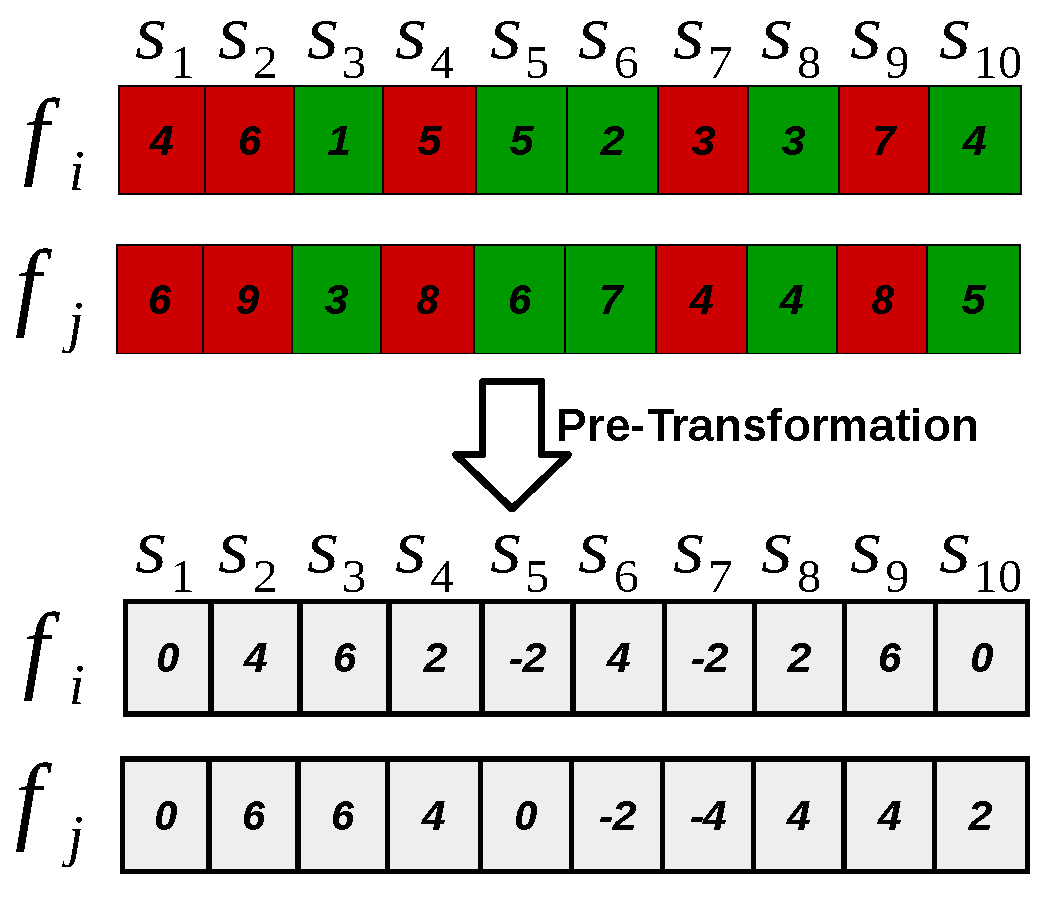
\includegraphics[width=\linewidth]{fig/transformation.pdf}
%     \vspace{-5mm}
%     \caption{Pre-Transformation}%{$\theta_{i,j}^{\ell}$ with Different Lines}
%     \label{fig:transform}
%   \end{subfigure}
%   \begin{subfigure}{.235\textwidth}
%     \centering
%     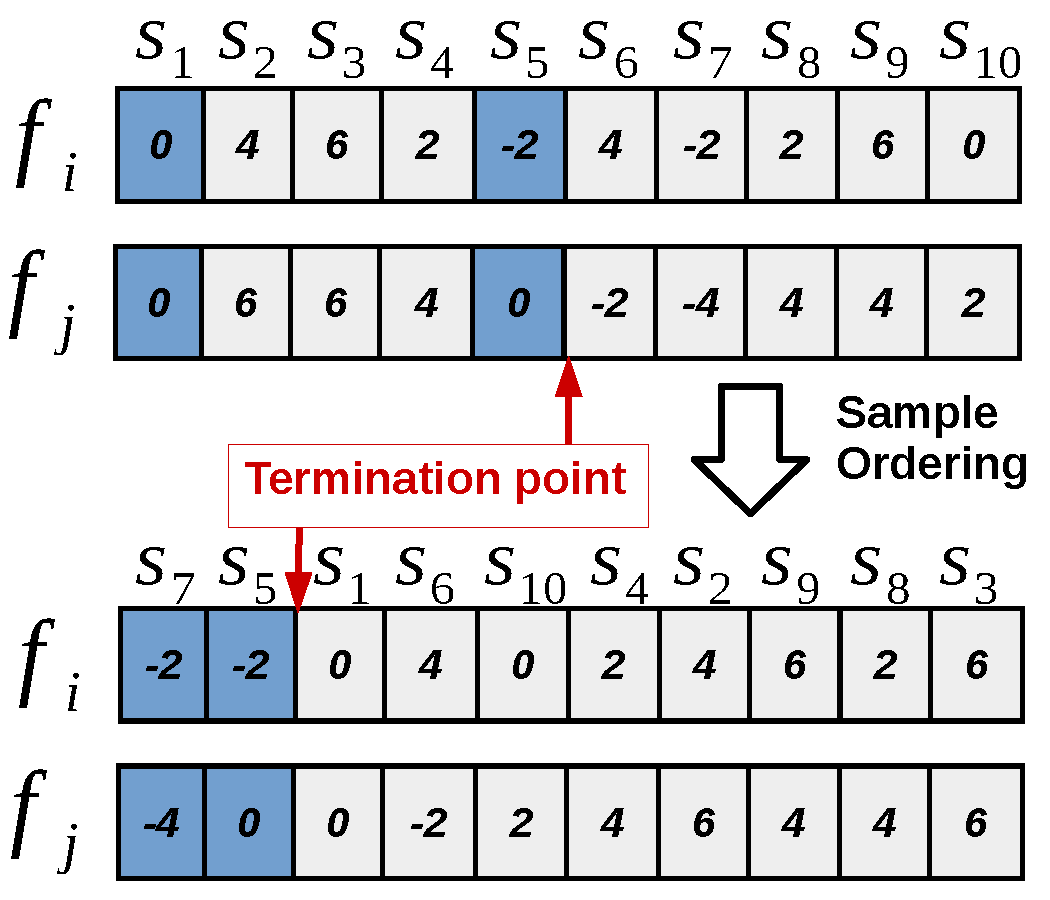
\includegraphics[width=\linewidth]{fig/earlyT.pdf}
%     \vspace{-5mm}
%     \caption{Early Termination ($\tau = 1$)}%{$\theta_{i,j}^{\hat{\ell}}$ with Representative Line}
%     \label{fig:earlyT}
%   \end{subfigure}
% \caption{Different Methods to Reduce Running Time}
% \label{fig:metric}
% \end{figure} 

\begin{figure}[h]
\centering     %%% not \center
\vspace{-5mm}
\subfigure[Pre-Transformation]{\label{fig:transform}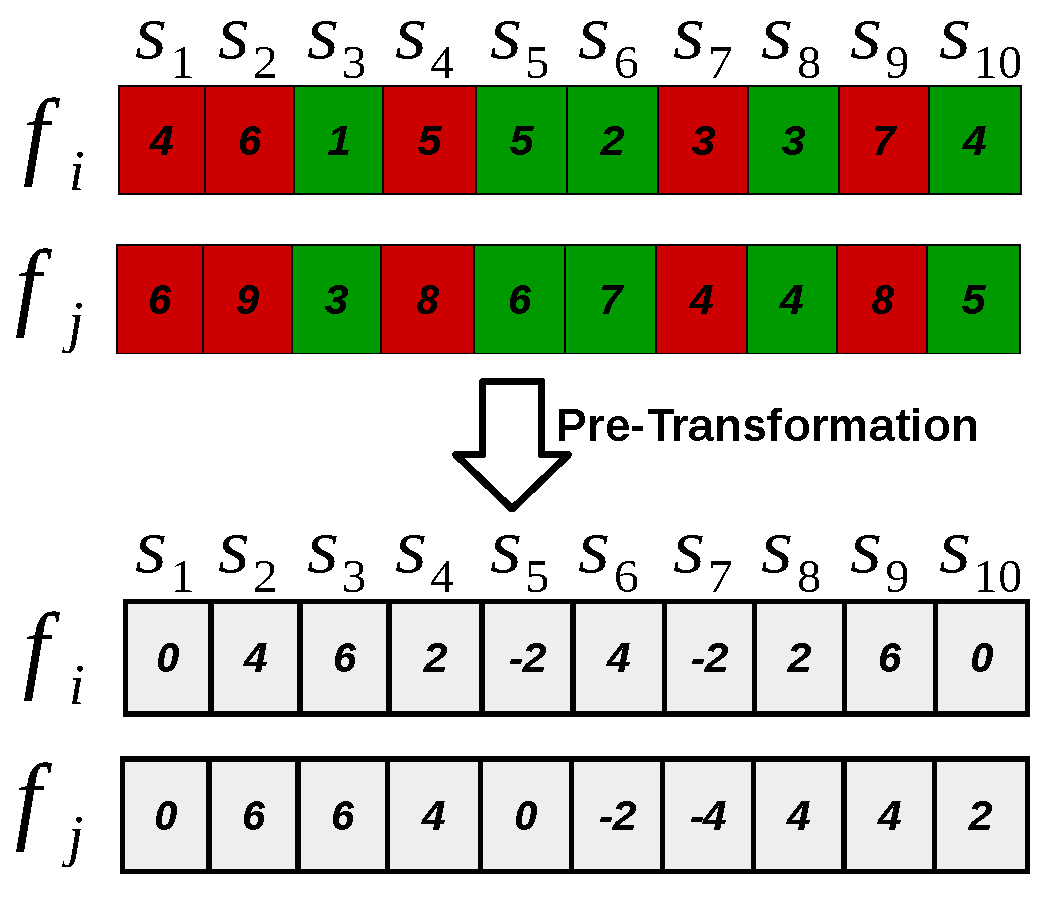
\includegraphics[width=.235\textwidth]{fig/transformation.pdf}}
\subfigure[Early Termination ($\tau = 1$)]{\label{fig:earlyT}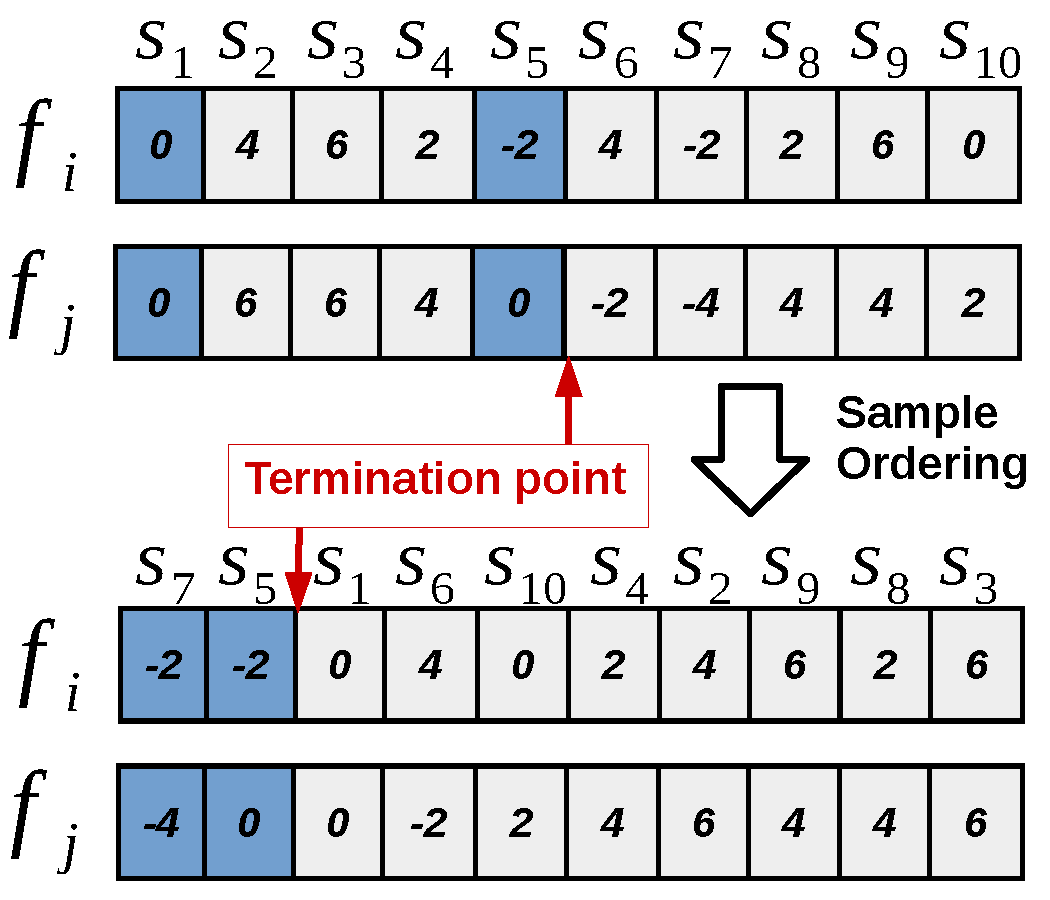
\includegraphics[width=.235\textwidth]{fig/earlyT.pdf}}
\vspace{-5mm}
\caption{Different Methods to Reduce Running Time}
\vspace{-5mm}
\label{fig:trans_term}
\end{figure}

% \begin{figure}[htbp]
% \centering
% \subfloat[first caption.\label{fig:1a}]{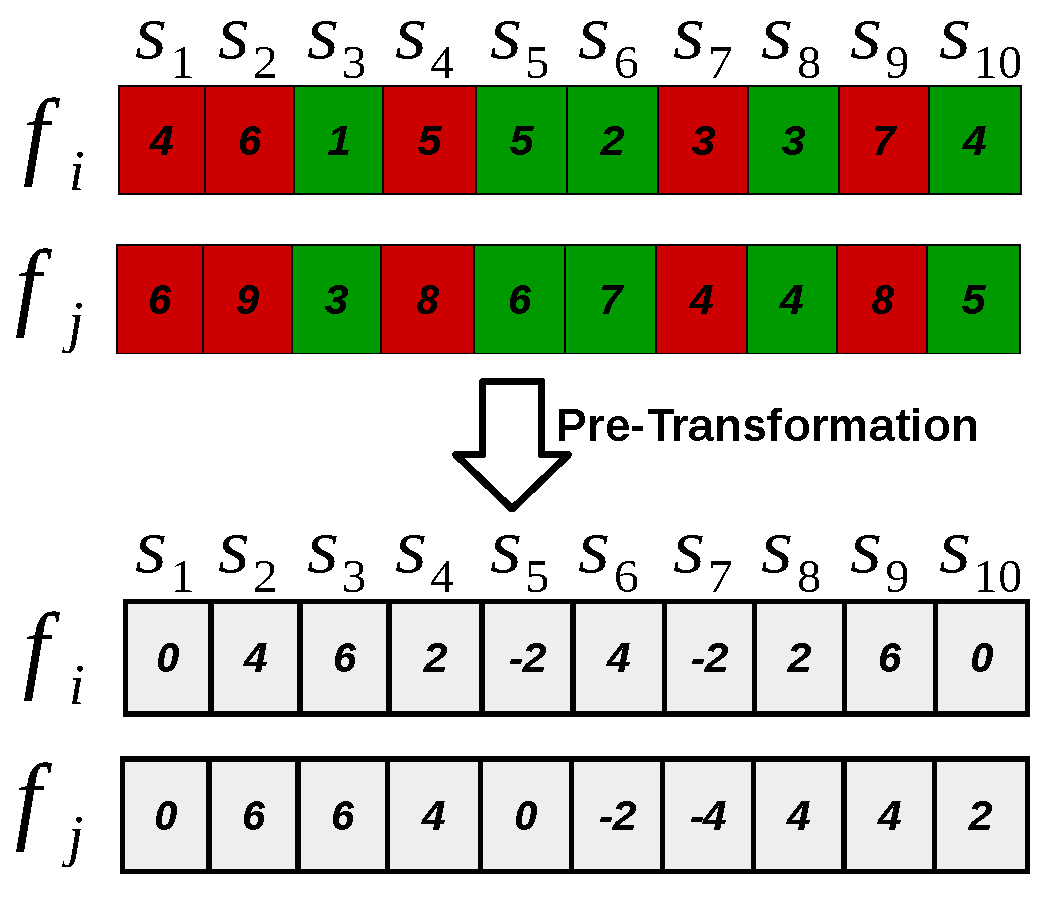
\includegraphics[width=0.2\textwidth]{fig/transformation.pdf}}\hfill
% \subfloat[second caption.\label{fig:1b}] {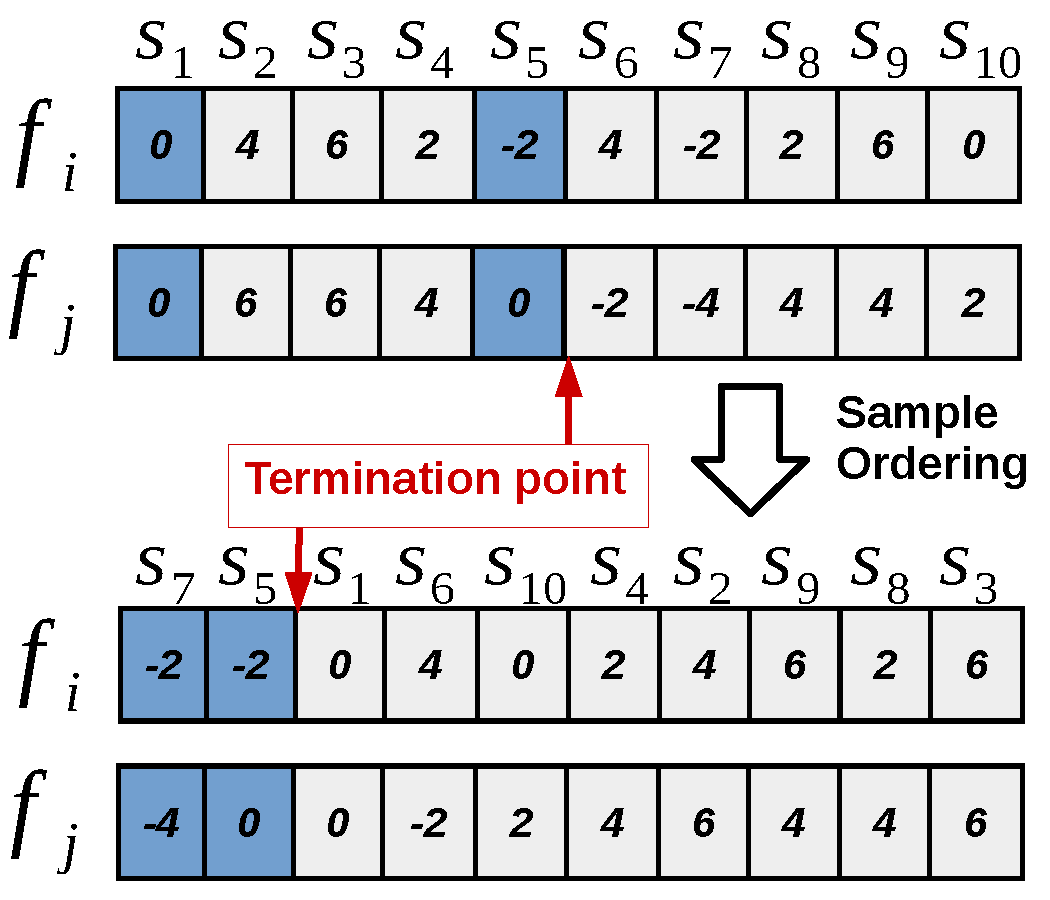
\includegraphics[width=0.185\textwidth]{fig/earlyT.pdf}}\hfill
% \end{figure}

\stitle{Remark.} For a feature pair $(f_i,f_j)$ where $i=j$, we can treat the corresponding $\theta_{i,i}$ as the separability score for a single feature $f_i$. Equation~\ref{eqn:s_object_transform} can be further reduced to Equation~\ref{eqn:s_object_transform_single}. Hence, we can calculate the separability score $\theta_{i,i}$ very efficiently for each single feature, based on the transformed matrix $\widehat{\mm}$.
\begin{equation}\label{eqn:s_object_transform_single}
\theta_{i,i}^{\hat{\ell},k}=\left\{
                \begin{array}{ll}
                  1 \textit{\hspace{2mm} if \hspace{2mm}} sign(\widehat{\mm}_{i,k}) = 1\\
                  0 \textit{\hspace{2mm} otherwise \hspace{2mm}} 
                \end{array}
              \right.
\end{equation}


\subsubsection{Early Termination} \label{ssec:earlyT}
Given a feature pair $(f_i,f_j)$, we need to make a full scan of all objects to compute the separability score $\theta_{i,j}^{\hat{\ell}}$ according to Equation~\ref{eqn:s_line}. However, we are not concerned about all feature pairs' separability score, instead we only care about the \topk feature pairs. Thus, we propose to reduce the running time using early termination when scanning the objects, denoted as \earlyT module as shown in Figure~\ref{fig:workflow}.

\stitle{High Level Idea.} The basic idea is to maintain a upper bound for the separability error of the \topk feature pairs, denoted as $\tau$. Correspondingly, the lower bound of separability score can be denoted as ($n-\tau$), where $n$ is the total number of objects $\hat{\oo}$. Given a feature pair $(f_i,f_j)$, we start to scan the object list until the number of mistakenly separated objects exceeds $\tau$, then terminate and prune this feature pair since it can not be among the \topk feature pairs; otherwise, $(f_i,f_j)$ is added to the \topk feature pair set and we update $\tau$ accordingly.

\stitle{Enhancement by Object Ordering.} Furthermore, in order to terminate early, an intuitive method is to first examine the objects that are more ``problematic''. In this way, given a bad feature pair, the number of mistakenly separated objects is likely to fast exceed $\tau$ by just looking at the first few objects. Hence, we propose to order the objects in descending order in terms the number of single features $f_i$ that separate this object $o_k$ mistakenly, i.e., $\widehat{\mm_{i,k}}\leq0$.

\begin{example}[\earlyT \& Object Ordering]
Figure~\ref{fig:earlyT} illustrates how early termination and object ordering help reduce the running time. The upper part is $\widehat{\mm}$ after transformation. Assume the current error upper bound is $\tau=1$. We start scan the object list from left to right and determine whether each object is correctly separated based on Equation~\ref{eqn:s_object_transform}. Object $o_1$ is mistakenly separated since $\widehat{\mm_{i,1}}+\widehat{\mm_{j,1}}\leq0$, marked as blue color in Figure~\ref{fig:earlyT}. We can terminate at $o_5$ since the number of mistakenly separated objects exceeds $\tau=1$.

The lower part of Figure~\ref{fig:earlyT} shows the $\widehat{\mm}$ after object reordering, where "problematic" objects are placed in the front. In this way, by only checking the first two objects, we can terminate and prune this feature pair.
\end{example}

\subsubsection{Sampling-based Estimation} \label{ssec:sampling}
We have proposed \earlyT module in Section~\ref{ssec:earlyT} to reduce the number of objects checked (i.e., $n$). However, there is no guarantee for the running time performance since the termination point is very data-dependent. In this section, we propose a stochastic method to reduce the number of examined objects, called \sampling. Instead of calculating $\theta_{i,j}$ over the whole object set $\hat{\oo}$, \sampling works on a sample set drawing from $\hat{\oo}$.

\stitle{High Level Idea.} At a high level, \sampling mainly consists of two phases, called {\em candidate generation} and {\em candidate validation} as shown in Figure~\ref{fig:sampling}. In phase one (Figure~\ref{fig:sampling}(a)), we estimate $\theta_{i,j}$ for each feature pair using a sampled set, and then generate the candidate feature pairs for full evaluation based on their confidence interval. In phase two (Figure~\ref{fig:sampling}(b)), we evaluate only the feature pairs in the candidate set, calculating $\theta_{i,j}$ over the whole object set $\hat{\oo}$ to obtain the final \topk feature pairs. %We will describe in detail in Section~\ref{sssec:generate} and \ref{sssec:validate}.
\begin{figure}[t!]
  \centering
  \vspace{-2mm}
  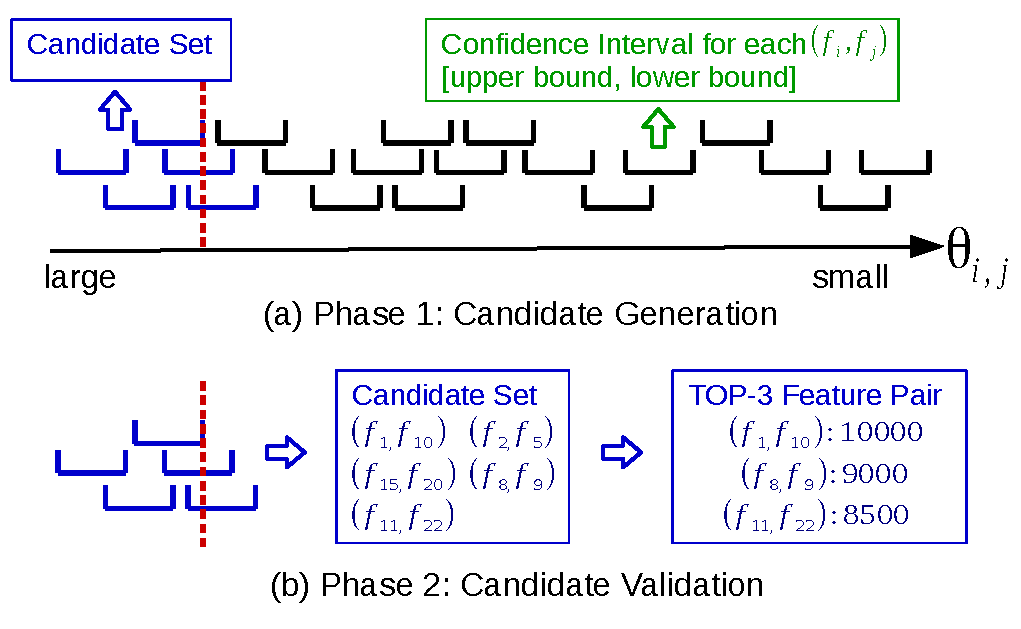
\includegraphics[width=\linewidth]{fig/sampling.pdf}
  \vspace{-9mm}
\caption{\sampling (TOP-3 Feature Pairs)}
\vspace{-5mm}
\label{fig:sampling}
\end{figure} 
% \begin{figure}[h]
%   \centering
%   \begin{subfigure}{0.235\textwidth}
%     \centering
%     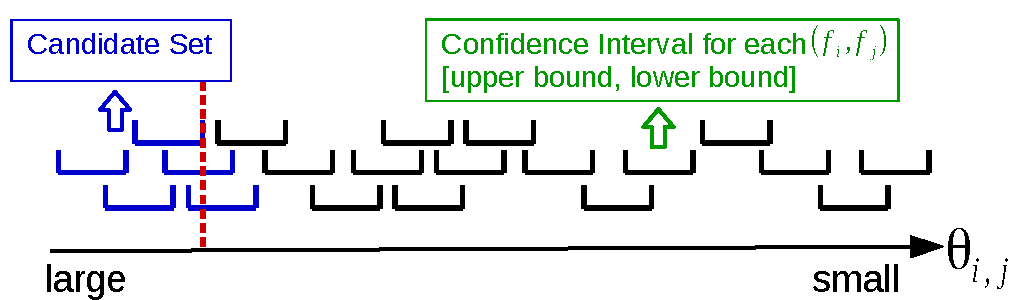
\includegraphics[width=\linewidth]{fig/phase1.pdf}
%     \vspace{-5mm}
%     \caption{Candidate Generation}%{$\theta_{i,j}^{\ell}$ with Different Lines}
%     \label{fig:phase1}
%   \end{subfigure}
%   \begin{subfigure}{.235\textwidth}
%     \centering
%     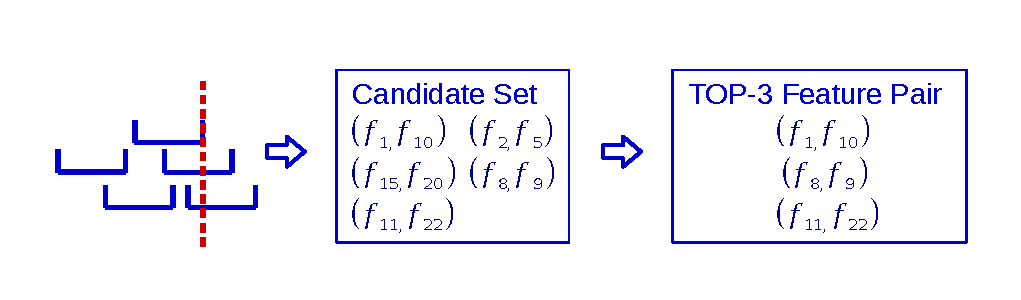
\includegraphics[width=\linewidth]{fig/phase2.pdf}
%     \vspace{-5mm}
%     \caption{Candidate Validation)}%{$\theta_{i,j}^{\hat{\ell}}$ with Representative Line}
%     \label{fig:phase2}
%   \end{subfigure}
% \caption{\sampling (TOP-3)}
% \label{fig:sampling}
% \end{figure} 

\stitle{Candidate Generation.} %\label{sssec:generate}
Let $\sss$ be the sample set drawn uniformly from the object set $\hat{\oo}$. Given a feature pair $(f_i,f_j)$, let $\theta_{i,j}(\sss)$ be the number of correctly separated objects in $\sss$. Let $\tilde{\theta}_{i,j}$ be the estimated separability score based on the sample set $\sss$. First, we can estimate $\tilde{\theta}_{i,j}$ from $\theta_{i,j}(\sss)$ using Equation~\ref{eqn:est_score}: the ratio of correctly separated samples is the same as that in $\hat{\oo}$. 

\begin{equation}\label{eqn:est_score}
\tilde{\theta}_{i,j} = \frac{\theta_{i,j}(\sss)}{|\sss|} \cdot n
\end{equation}

Next, we will show that with a constant sample set size $|\sss|$, $|\theta_{i,j}-\tilde{\theta}_{i,j}|$ is bounded by a small value with high probability. 

\begin{theorem}[Estimation Accuracy~\cite{acharya2015fast}]\label{them:est}
By considering $\Omega(\frac{1}{\epsilon^2}\cdot \log(\frac{1}{\delta}))$ samples, with probability at least $1-\delta$, we have $|\frac{\theta_{i,j}(\sss)}{|\sss|}-\frac{\theta_{i,j}}{n}| \leq \epsilon$, i.e., $|\tilde{\theta}_{i,j}-\theta_{i,j}|\leq \epsilon n$.
\end{theorem}

We can treat $log(1/\delta)$ as a constant, e.g., by setting $\delta = 0.05$.Thus, Theorem~\ref{them:est} essentially states that with only $\Omega(\frac{1}{\epsilon^2})$ samples, with probability 95\% the confidence interval for $\theta_{i,j}$ is $[\tilde{\theta}_{i,j}-\epsilon n, \tilde{\theta}_{i,j}+\epsilon n]$. Note that the sample size $|\sss|$ only relies on $\epsilon$ and is independent of the object size $n$. Hence, the \sampling module helps \genviz scale to datasets with large $n$. 
%For instance, when setting $\epsilon=0.05$, the sample size is fixed to be $400$. 

With Theorem~\ref{them:est}, we can first calculate the confidence interval of $\theta_{i,j}$ for each feature pair $(f_i,f_j)$, as shown in Figure~\ref{fig:sampling}(a). Next, we compute the lower bound of $\theta_{i,j}$ for the \topk feature pairs, denoted as $\zeta$ as shown by the red dotted line in Figure~\ref{fig:sampling}(a). At last, we can prune away feature pairs whose upper bound is smaller than $\zeta$. Accordingly, the candidate set $\cc$ corresponds to the feature pairs depicted by the blue intervals in Figure~\ref{fig:sampling}(a). These feature pairs $\cc$ will be further validated in phase two, i.e., candidate validation. Typically, $|\cc|$ is orders of magnitude smaller than $m^2$, the original search space for all feature pairs. We will verify this later in our experiments (Section~\ref{sec:exp}). 

\begin{example}[Candidate Generation]
Let us illustrate phase one using Figure~\ref{fig:sampling}(a). Set $\epsilon = 0.05$ and $K=3$. We sample $\Omega(\frac{1}{\epsilon^2})=400$ objects and compute the confidence interval of $\theta_{i,j}$ for each $(f_i,f_j)$. Next, we obtain the $3^{th}$ lower bound $\zeta$ (red dotted line) in descending order among all the confidence intervals. At last, we generate the blue feature pair candidates $\cc$, whose upper bound is larger than the red dotted line.
\end{example}

\stitle{Candidate Validation.} %\label{sssec:validate}
In phase two, we re-evaluate all the feature pair candidates generated from phase one. The evaluation is performed on the whole object set $\hat{\oo}$. For each feature pair $(f_i,f_j)\in \cc$, we calculate the real separability score $\theta_{i,j}$, and find the \topk feature pairs as shown in Figure~\ref{fig:sampling}(b). 
\begin{figure}[h]
  \centering
  \vspace{-5mm}
  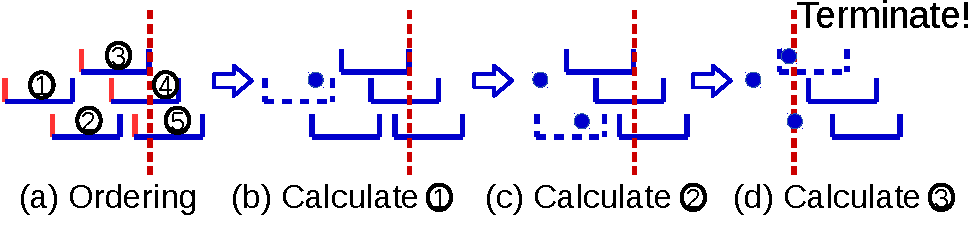
\includegraphics[width=\linewidth]{fig/candidate_ordering.pdf}
  \vspace{-6mm}
\caption{Enhancement by Candidate Ordering}
\vspace{-5mm}
\label{fig:candidate_ordering}
\end{figure} 

\stitle{Enhancement by Candidate Ordering.}  Instead of naively validating each feature pair candidate, we further propose to first order the candidates in descending order of the upper bound of each confidence interval. Then, we sequentially calculate the real separability score $\theta_{i,j}$ for each feature pair, and update $\zeta$ correspondingly. Recall that $\zeta$ is the maintained lower bound of $\theta_{i,j}$ for the \topk feature pairs. At last, we terminate when the feature pair's upper bound is even smaller than the current $\zeta$.


\begin{example}[Candidate Ordering]
We illustrate it using Figure~\ref{fig:candidate_ordering}. Initially, the lower bound of the \topthree feature pairs, i.e., $\zeta$, is depicted using the red dotted line  in Figure~\ref{fig:candidate_ordering}(a). We first sort the feature pair candidates in descending order of the upper bound (red line). Next, we calculate $\theta_{i,j}$ for the first feature pair, as shown by the blue ball in Figure~\ref{fig:candidate_ordering}(b), with $\zeta$ unchanged. Similarly, we calculate $\theta_{i,j}$ for the second and third feature pairs, as shown in Figure~\ref{fig:candidate_ordering}(c) and (d), and update $\zeta$ accordingly. Note that $\zeta$ (the red dotted line) is moved forward in Figure~\ref{fig:candidate_ordering}(d). Since $\zeta$ is already larger than the upper bound of the following feature pair, we can terminate.
\end{example}

\subsubsection{Search Space Traversal} \label{ssec:traversal}
In Section~\ref{ssec:earlyT} and \ref{ssec:sampling}, we have discussed how to reduce the number of objects checked (i.e., $n$). The question followed is that can we reduce the number of feature pair considered (i.e., $m^2$). In this section, we focus on how to smartly traverse the search space if allowed only a limited number of feature pairs, called \traversal module. 

\stitle{High Level Idea.}  The basic idea is that instead of examining each possible feature pair, we only check a limited number of feature pairs, but in a {\em smarter traversal order}. The number of checked feature pairs determines a trade-off between the efficiency and the accuracy. In general, the less number of feature pairs checked, the faster in terms of the running time, however, at the cost of accuracy in terms of the output \topk feature pairs. 

The full search space for the feature pairs is the upper triangle in Figure~\ref{fig:traversal}(a), where each row represents $f_i$ and each column represents $f_j$. Let $\chi$ be the limited number of feature pairs to be checked. We propose two different traversal order over the search space: horizontal traversal and vertical traversal. In the following, we will describe them in detail.
\begin{itemize}
\item \emph{Horizontal traversal (Figure~\ref{fig:traversal}(a)):} for each feature $f_i$, pair it with each other feature $f_j$, where $j\geq i$, and obtain $(f_i,f_j)$. Repeat it for each $f_i$, where $1 \leq i\leq m$.
\item \emph{Vertical traversal (Figure~\ref{fig:traversal}(b)):} for each feature $f_j$, pair it with each other feature $f_i$, where $i\leq j$, and obtain $(f_i,f_j)$. Repeat it for each $f_j$, where $1 \leq j\leq m$.
%\item \emph{Diagonal traversal (Figure~\ref{fig:traversal}(c)):} for a fixed value $v$, pair $(f_i,f_{v-i})$, where $1\leq i<v$. Repeat it for each $v$, where $2 \leq v\leq 2m$.
\end{itemize}

\begin{figure}[h]
  \centering
  \vspace{-5mm}
  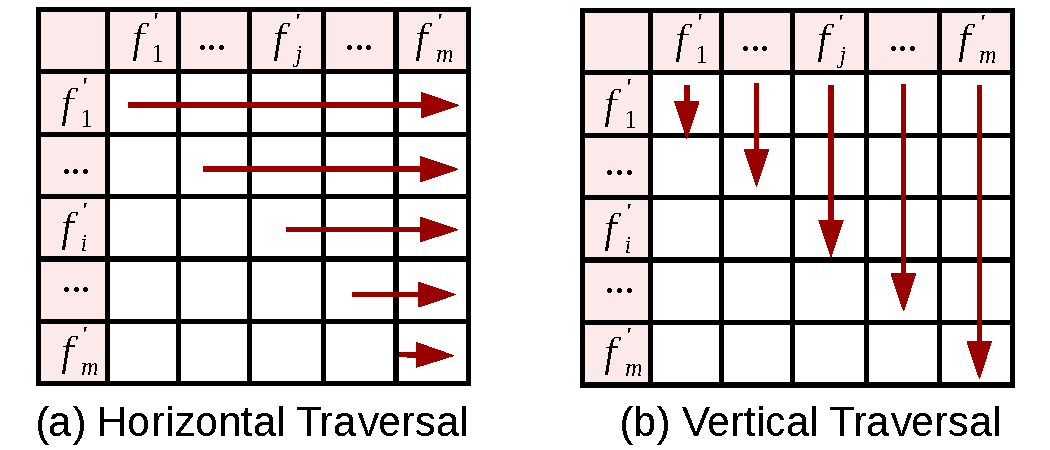
\includegraphics[width=0.85\linewidth]{fig/traversal.pdf}
  \vspace{-5mm}
\caption{Different Traversal Ordering}
\vspace{-5mm}
\label{fig:traversal}
\end{figure} 

However, the traversal order does not convey any intuition if the feature set $\ff$ is in random order. Hence, we further propose to enhance \traversal by feature ordering in $\ff$.

\stitle{Enhancement by Feature Ordering.} We propose to first sort features based on single feature's separability score $\theta_{i,i}$. Single features with good performance individually, i.e., with high separability score, are ranked first. Let $\{f_1^{'} f_2^{'},\cdots,f_m^{'}\}$ be the sorted single feature set. Next, we discuss the intuition behind different traversal order scheme. We coarsely classify the sorted feature set into three categories based on the single feature separability score $\theta_{i,i}$: {\em top, median,} and {\em bad}. 

\begin{itemize}
\item \emph{Horizontal traversal:} the intuition is that there is at least one {\em top} or {\em median} single feature in each \topk feature pair $(f_i,f_j)$.
\item \emph{Vertical traversal:}  the intuition is that both features in each \topk feature pair $(f_i,f_j)$ must rank {\em top} or {\em median} individually.
%\item \emph{Diagonal traversal:} 
\end{itemize}


%The intuition behind horizontal traversal is that there is at least one {\em top} or {\em median} single features in the \topk feature pairs $(f_i,f_j)$; while the intuition behind  horizontal traversal is that both features in \topk feature pairs $(f_i,f_j)$ must rank {\em top} or {\em median} by their own.

%Typically, $K$ is not large, e.g., {\sc Top-1000}, while $m$ is large, e.g., {\sc 20000}. 
\begin{example}[\traversal]
Assume $m=2\times 10^4$ and $K=100$. Set $\chi=10^7$. Initially, the number of possible feature pairs is $\frac{m^2}{2}=2\times 10^8$; but we reduce the whole search space to  $\frac{1}{20}$ of that size,  i.e., $\chi=10^7$. First, single features are sorted in descending order of their individual separability score. In horizontal traversal, only feature pairs, with at least one individual feature ranked in the top 500, are considered; while in vertical traversal, only feature pairs, with both individual features ranked better than 2000, are considered.
%the "worst" $f_i$ ranks around 500, while $f_j$ can be any feature in $\ff$. On the other hand, in vertical traversal, the "worst" $f_i$ (and $f_j$) ranks around 2000.
\end{example}



%==================================================================
\section{Results}
\label{sec:exp}
In this section, we first describe the datasets and algorithms used in our evaluation. Next, we test the running time and separability quality with different algorithms. Lastly, we compare \topk feature pairs with \topk single features, and justify the necessity of using feature pairs instead of single features.
\subsection{Experimental Setup}
\begin{table}[h]
\centering
\vspace{-5mm}
\small
\begin{tabular}{|c|c|c|c|c|c|c|c|c|}
  \hline
    &  $|\ff|$=$m$ & $|\oo|$=$N$ & $|\sss|$ & $\chi$  & \# of $\widehat{\oo}$ & avg($|\oo_+|$) & avg($|\oo_-|$) \\
  \hline
  \msig  & 19,912 & 22,209 & 400 & $10^7$ & 10 & 295 & 21,914 \\
    \hline
  \lincs  & 22,268 & 98,061 & 400 & $10^7$ & 40 & 165 & 97,897 \\
    \hline
 \end{tabular}
\caption{Dataset Statistics}
\label{tbl:dataset}
\vspace{-18pt}
\end{table}

\stitle{Dataset.} We conduct experiments on two different biological applications called \msig and \lincs.  In the \msig application, we are given a feature-object matrix with genes as the objects and different gene set properties as the features.  The scores in the matrix represent the stationary probability of reaching the object gene node in a random walk on a heterogenous network that restarts at the feature gene set property node [CITE DRAWR].  The heterogenous network here was constructed with information from BLAST, Gene Ontology, Pfam, and …  . The positive object sets for each experiment in \msig is a set of differentially expressed genes in a high-profile cancer study that was curated by the Molecular Signatures Database [CITE MSIGDB].  In the \lincs application, our feature-object matrix contains imputed expression z-scores for different genes (features) across many drug experiments (objects) conducted on the MCF7 cell line by the LINCS L1000 project [CITE].  The positive object sets for \lincs are multiple experiments that used the same small molecule perturbagen, although at varying dosages and durations. \silu{TODO:LINCs and MsigDB description}
For each of the two applications, the number of features $m$, objects $N$, sample size $|\sss|$, and the examined feature pairs $\chi$ are depicted in Table~\ref{tbl:dataset}.
We tested on 10 different cancer gene sets for \msig and 40 different drug experimental sets for \lincs as shown by "\# of $\widehat{\oo}$" in Table~\ref{tbl:dataset}. For each of positive object set, we treat all remaining objects as the negative set and list the average number of positive and negative objects in Table~\ref{tbl:dataset}. Note that the average number of positive objects is far less than the average number of negative objects. In order to balance between the number of positive objects and negative objects, we adjust Equation~\ref{eqn:s_line} to a weighted sum form as shown in Equation~\ref{eqn:s_line_weighted}.

\begin{equation}\label{eqn:s_line_weighted} 
\hspace{3mm} \theta_{i,j}^{\ell}= \sum_{o_k\in{\oo_-}}{\theta_{i,j}^{\ell,k}}+\frac{|\oo_-|}{|\oo_+|}\cdot\sum_{o_k\in{\oo_+}}{\theta_{i,j}^{\ell,k}} %{\sf Separability \hspace{1mm} Score\hspace{1mm} with\hspace{1mm} Line\hspace{1mm} \ell:}
\end{equation}

\begin{table*}[t]
\centering
\small
\begin{tabular}{|c|c|c|c|c|c|c|c|c|}
  %\hline

  \hline
   &  Transformation & \earlyT & Object Ordering & \sampling & Candidate Ordering & \traversal & Feature Ordering & Complexity\\
  \hline
  \baseline  & yes & no  & no & no & no & Any & no & $O(m^2n)$\\
    \hline
  %\early  & yes & yes  & no & no & no & Any & no & $O(m^2n)$\\
   % \hline
  \earlyOrder & yes & yes  & yes & no & no & Any & no & $O(m^2n)$\\
    \hline
  \samp  & yes & no  & no & yes & no & Any & no & $O(mn+m^2|\sss|+|\cc|n)$\\
    \hline
  \sampOpt  & yes & no  & no & yes & yes & Any & no & $O(mn+m^2|\sss|+|\cc|n)$\\
    \hline
  \horiz  & yes & no  & no & yes & yes & Horizontal & yes & $O(mn+\chi|\sss|+|\cc|n)$\\
    \hline
  \vertic  & yes & no  & no & yes & yes & Vertical & yes & $O(mn+\chi|\sss|+|\cc|n)$ \\
    \hline
 \end{tabular}
\caption{Algorithms Using Different Optimization Modules}
\label{tbl:alg}
\vspace{-18pt}
\end{table*}


\stitle{Algorithm.} In our evaluation, we experimented with different combinations of the optimization modules introduced in Section~\ref{sec:opt} and present the combinations listed in Table~\ref{tbl:alg}. Some combinations are always inferior to others and are not listed in Table~\ref{tbl:alg}, e.g. the unlisted algorithm with only \trans and \earlyT modules  always has a worse running time and the same separability quality as the listed \earlyOrder. We use the algorithm with only \trans module as \baseline. The last column in Table~\ref{tbl:alg} shows the running time complexity of different algorithms, where $m$ and $n$ are constants, $|\sss|$ and $\chi$ are predetermined, while $|\cc|$ is generated during the algorithm and can be different among the last four rows in Table~\ref{tbl:alg}. Take \horiz as an example: first, \trans module takes $O(mn)$; second, \traversal module requires a sorting over the feature set, taking $O(m\log m)$\footnote{Since $m\log m < nm$, we omit term $m\log m$ from the overall complexity.}; last, with \sampling modules over $\chi$ feature pairs, the running time is reduced from $O(m^2n)$ to $O(\chi|\sss|+|\cc|n)$, where the first and second term represent the time for candidate generation and candidate validation respectively. Note that $|\cc|$ is typical orders of magnitude smaller than $\chi$ in \horiz as discussed in Section~\ref{ssec:sampling}. 

\subsection{Comparison of Different Algorithms}
In this section, we compare the performance of different algorithms in terms of the running time and the separability quality for top-1000 feature pairs. We illustrate the results using boxplots\footnote{Boxplot: https://en.wikipedia.org/wiki/Box\_plot. Whisker is set to be 1.5 IQR.} in Figure~\ref{fig:time} and \ref{fig:separability}. 



\stitle{Running Time.} Figure~\ref{fig:time} depicts the running times of different algorithms. Each box corresponds to one algorithm, representing the running time's distribution among all object sets (i.e., 10 for \msig and 40 for \lincs). 
To aid comparison, we explicitly record the median of each algorithm with the tick label in the upper part of Figure~\ref{fig:time}, corresponding to the horizontal line in the filled box. Additionally, the average running time is marked with a star point in the box for each algorithm. First, let us compare the median running time among different algorithms. For \msig, \baseline takes more than 2 hours, \earlyOrder takes less than 1 hour, \samp and \sampOpt take around 6 and 5 min respectively, while \horiz and \vertic both take only 1 min. We can see that \earlyT module helps achieve $2\times$ speed up; while \sampling module helps reduce the running time dramatically, with $20\times$ reduction from \baseline to \sampOpt. By checking around $\frac{1}{20}$ of all feature pairs, \horiz and \vertic only achieve around $6\times$ speed-up compared to \sampOpt. This is because: (a) \horiz and \vertic incur the feature ordering overhead (around $6s$), along with the transformation time (around $8s$); (b) during the candidate generation phase, \sampOpt is capable to prune more percentage of feature pairs than \horiz and \vertic, since on average the feature pairs considered in \horiz and \vertic are better than that in \sampOpt. Next, let us look at the interquartile range (IQR) for different algorithms. Remember that the y-axis in Figure~\ref{fig:time} is in log-scale. We can see that \earlyOrder has a very large interquartile range, indicating that \earlyT module is very data-dependent. As we discussed in Section~\ref{ssec:earlyT}, \earlyT has no guarantee on the improvement of the running time. Sometimes, it can be even worse than \baseline as shown in Figure~\ref{fig:lincs_time}, because \earlyT incurs the overhead of checking the pruning or terminating criteria when scanning the object list for each feature pair.
Similar results can be found in Figure~\ref{fig:lincs_time} for \lincs. In particular, the transformation and feature ordering overhead take $45+35=80s$ in \horiz and \vertic.

% (b) the pruning of feature pairs in candidate generation phase is more powerful in \sampOpt, since on average the feature pairs considered in \horiz and \vertic is better than that in \sampOpt intuitively.


\begin{figure}[h]
\centering     %%% not \center
\vspace{-5mm}
\subfigure[\msig]{\label{fig:msig_time}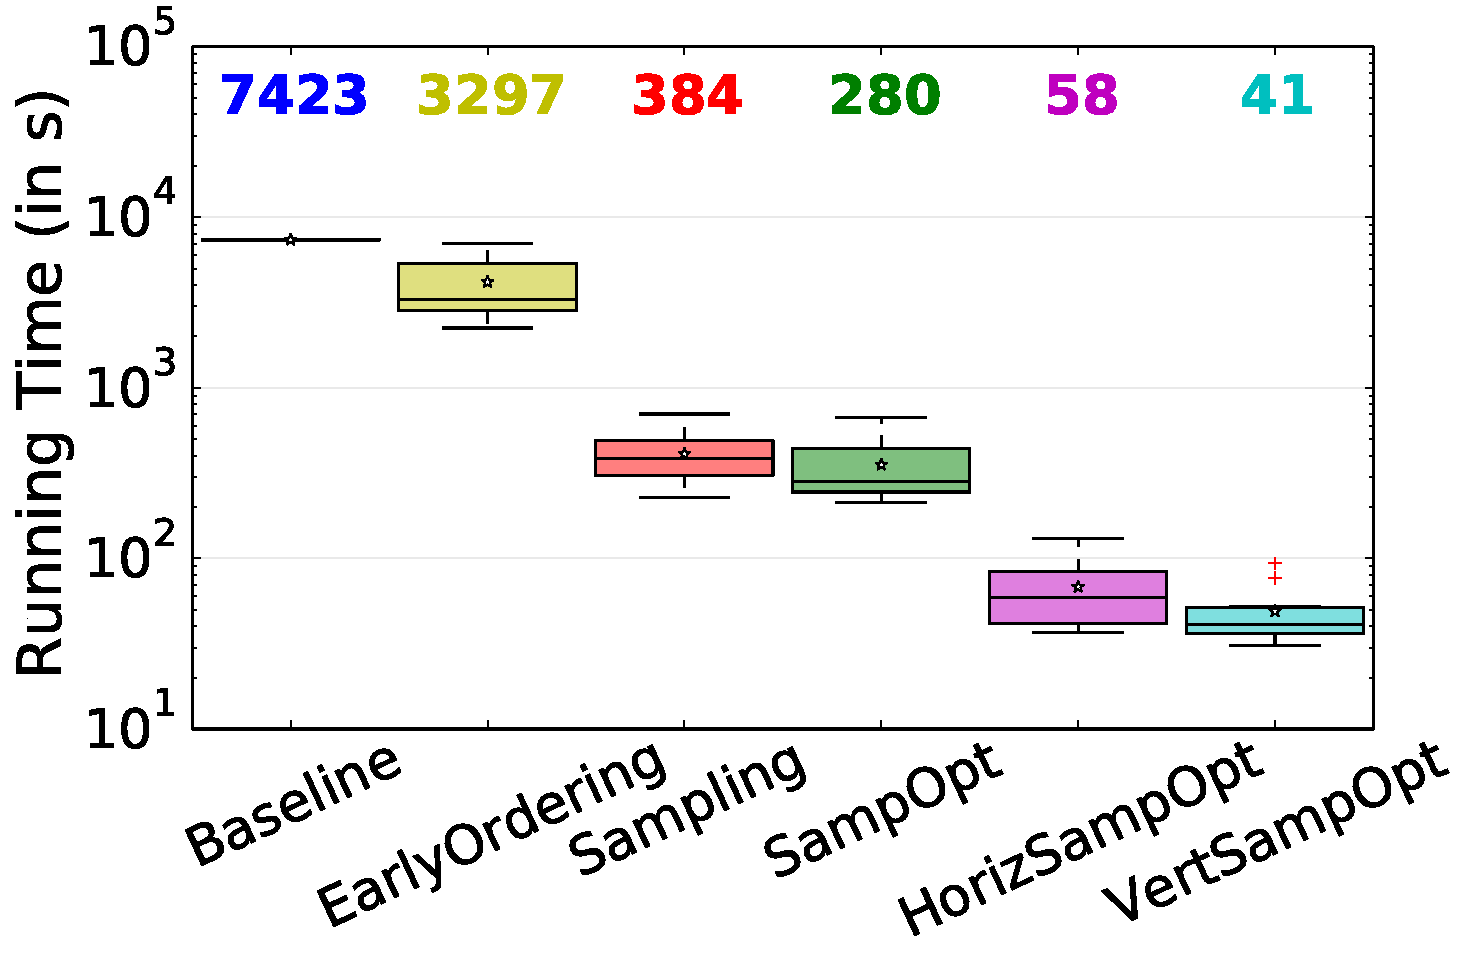
\includegraphics[width=.235\textwidth]{fig/msig_time.pdf}}
\subfigure[\lincs]{\label{fig:lincs_time}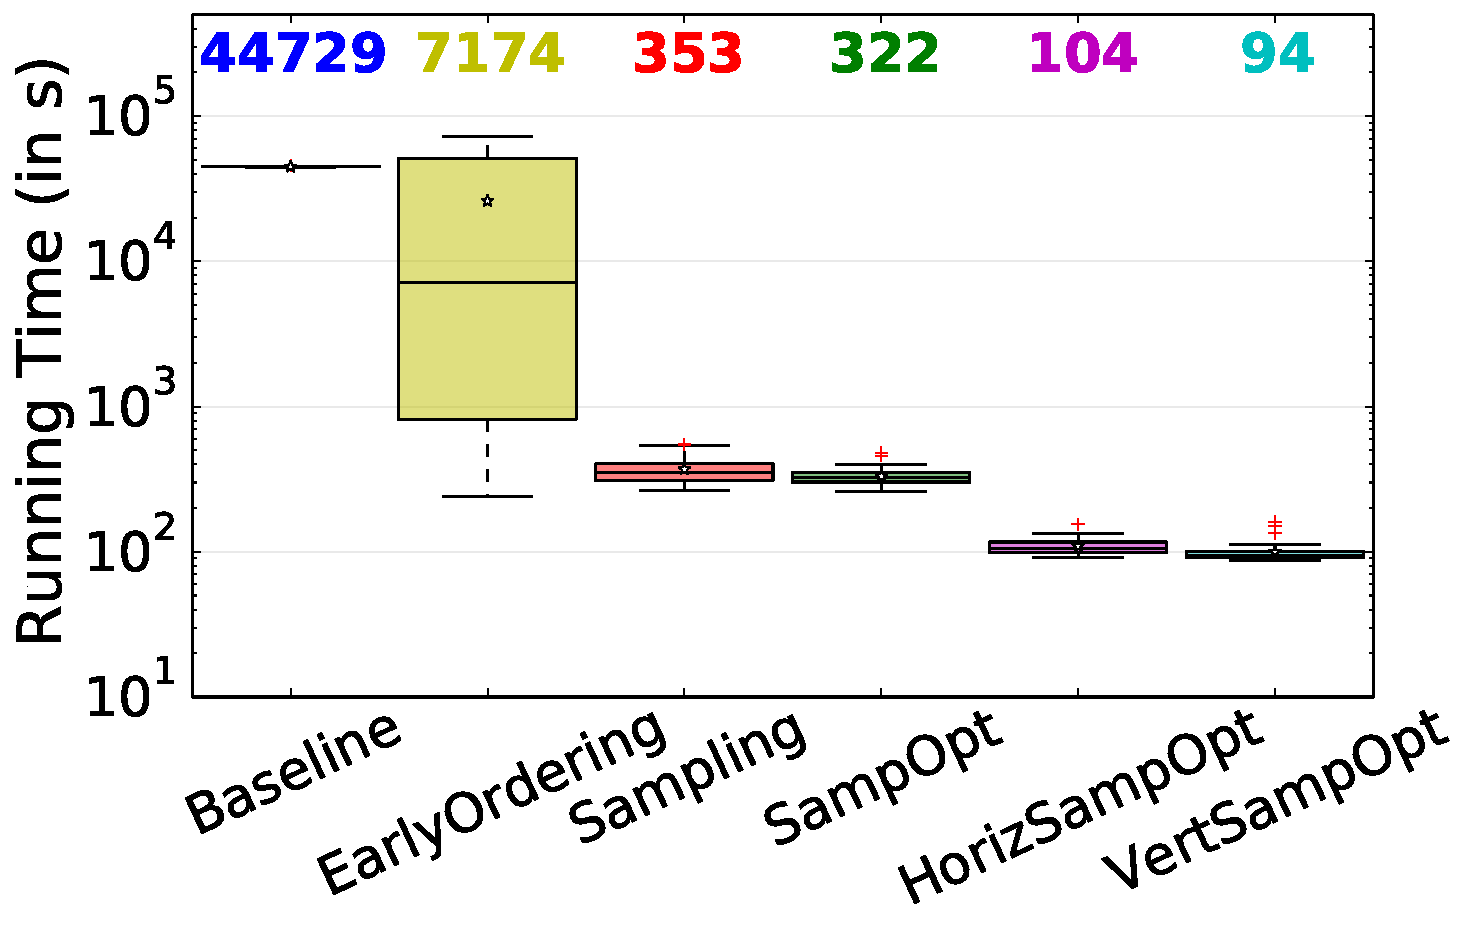
\includegraphics[width=.235\textwidth]{fig/lincs_time.pdf}}
\vspace{-5mm}
\caption{Running Time Comparison}
\vspace{-3mm}
\label{fig:time}
\end{figure}

\begin{figure}[h]
\centering     %%% not \center
\subfigure[\msig]{\label{fig:msig_separability}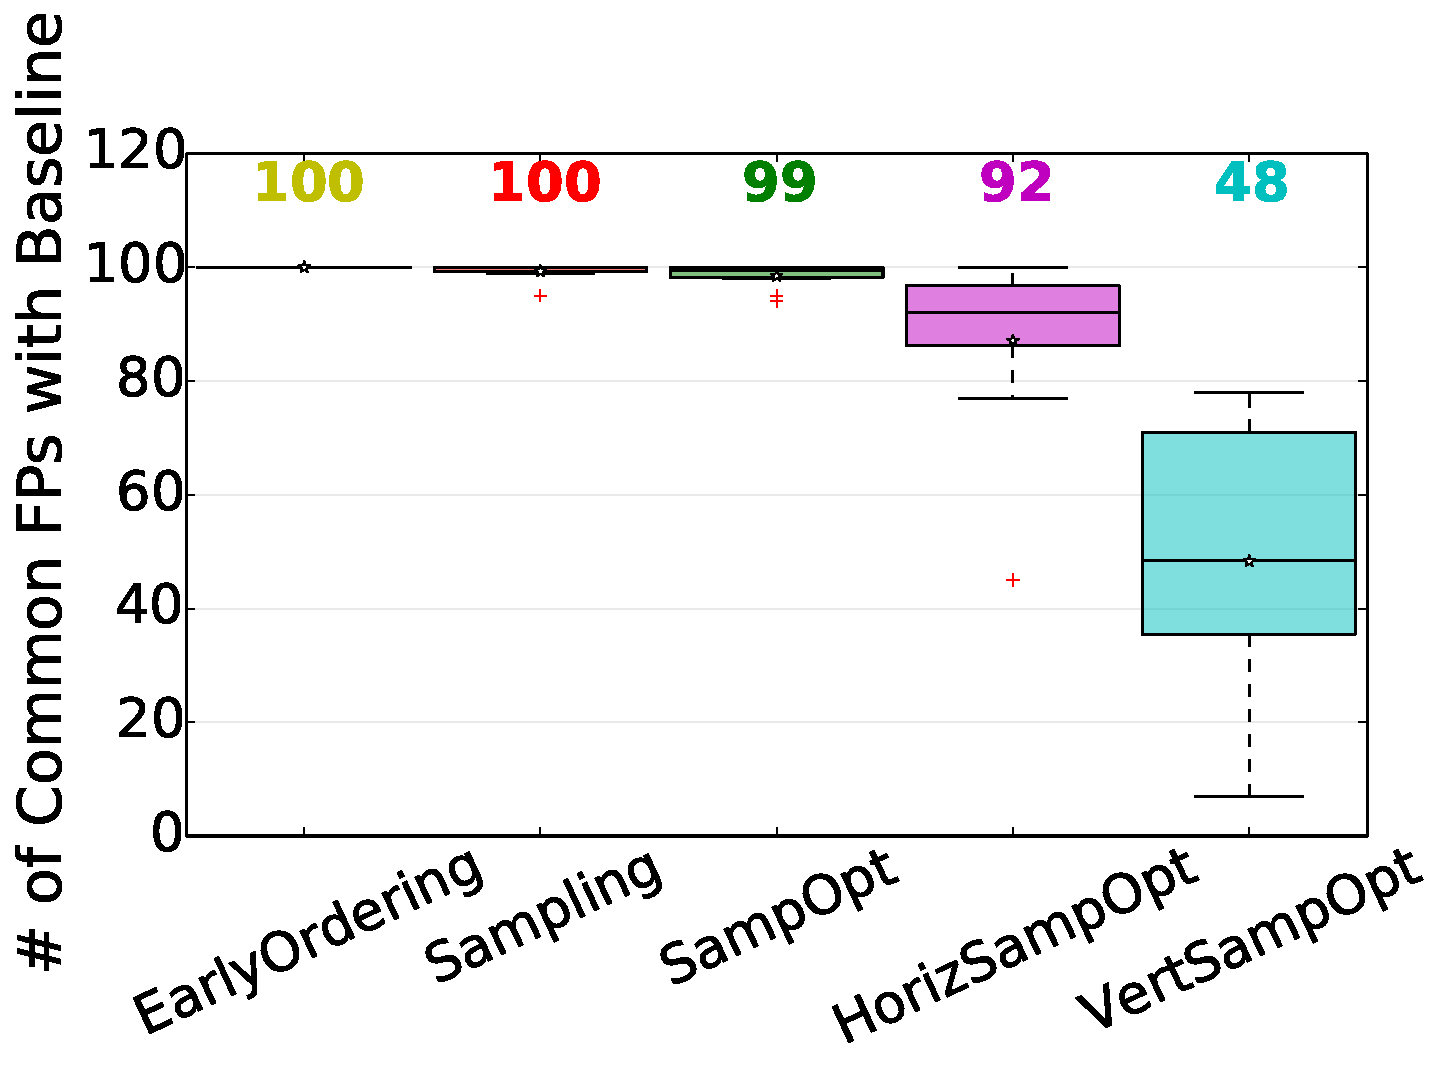
\includegraphics[width=.235\textwidth]{fig/msig_accuracy.pdf}}
\subfigure[\lincs]{\label{fig:lincs_separability}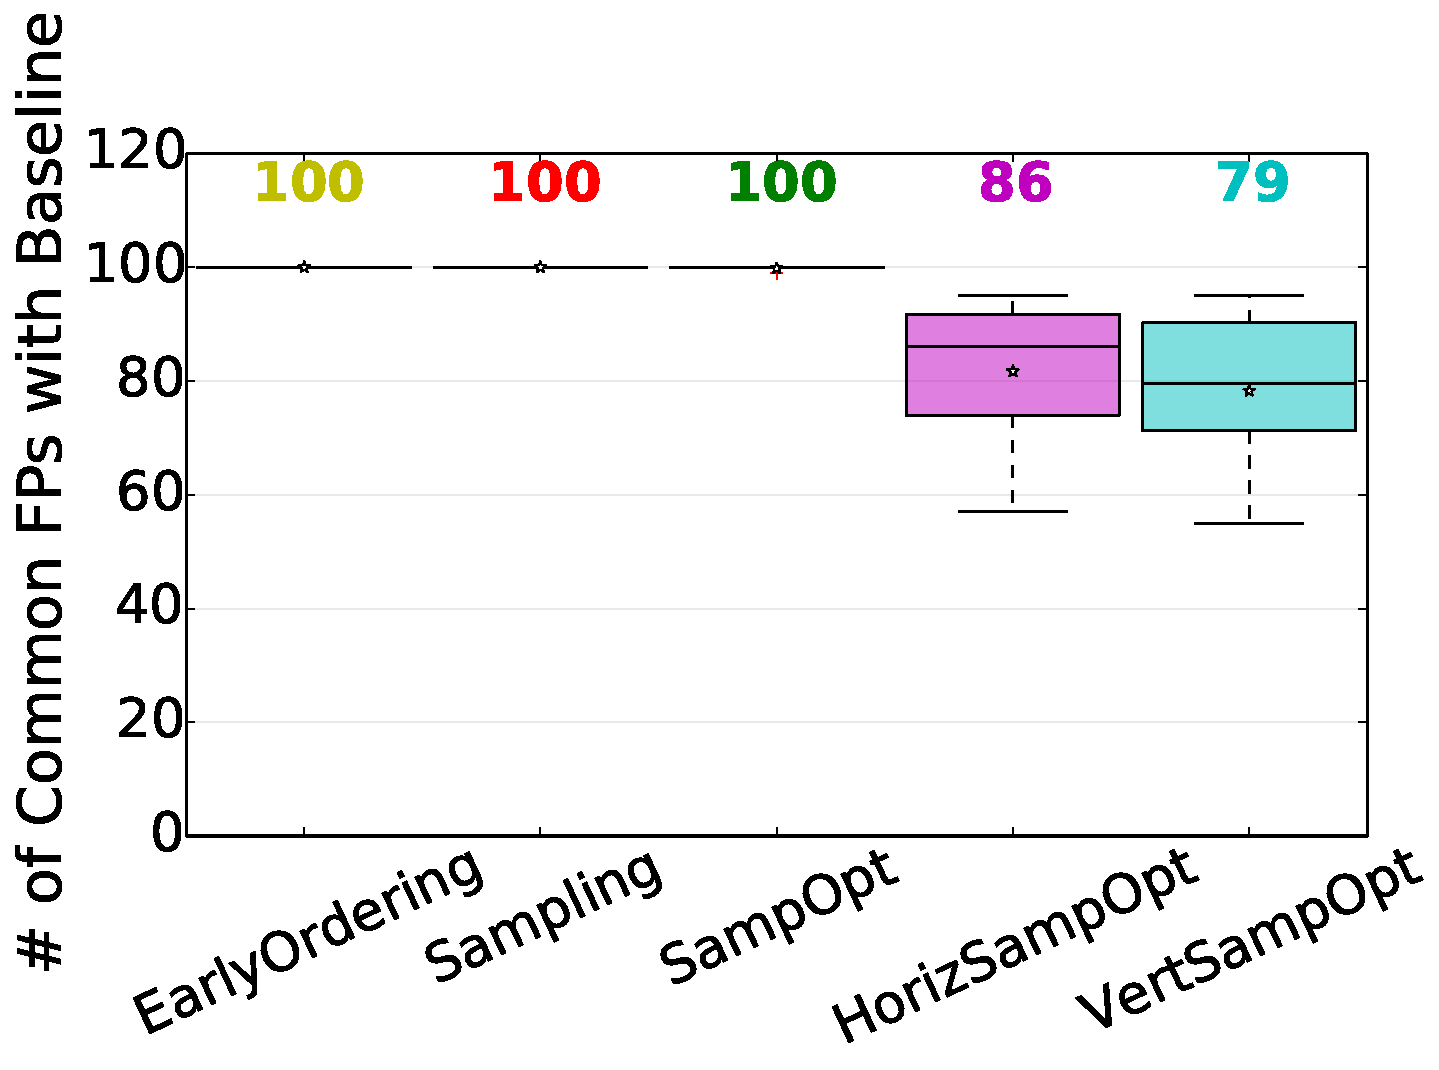
\includegraphics[width=.235\textwidth]{fig/lincs_accuracy.pdf}}
\vspace{-5mm}
\caption{Separability Quality Comparison}
\vspace{-5mm}
\label{fig:separability}
\end{figure}

\stitle{Separability Quality.} Recall that \earlyT module is deterministic and does not decrease the qualilty of the output \topk feature pairs; \sampling module is stochastic and has probabilistic guarantee on the output \topk feature pairs; and the \traversal module is heuristic and may output \topk feature pairs that are very different from \baseline. Given an algorithm, we measured the output quality using the number of common feature pairs returned by the \baseline and the given algorithm. Figure~\ref{fig:separability} depicts this separability quality comparison. Let us first focus on \msig. \earlyOrder has exactly the same output as \baseline. We also observe that \samp and \sampOpt share almost the same top-100 feature pairs with \baseline, thanks to the probabilistic guarantee as stated in Theorem~\ref{them:est}. \horiz and \vertic output a median of 92 and 48 feature pairs in common with \baseline respectively, because of the heuristic \traversal module. In general, \horiz is much better than \vertic, with higher median and smaller interquartile range as shown in Figure~\ref{fig:msig_separability}. This indicates that it is insufficient to just consider the top single features as in \vertic. The observation matches our motivation of finding feature pairs instead of single features.

\subsection{Feature Pair vs. Single Feature.}
In this section, we first calculated the p-value for each \topk single feature and feature pair, using Fisher's exact test on a $2\times2$ contingency table. This contingency table is obtained after executing the algorithm in Table~\ref{tbl:alg}, with rows being the true positive and negative label, the columns being the predicted positive and negative label, and the table values being the number of objects that belong to each cell. The p-value from Fisher's exact test represents the significance of deviation from the null hypothesis, i.e., the predicted label is independent of the real label. Next, we assert that feature pairs can provide better separability performance or new insights compared to single features: (a) {\em better:} feature pairs have improved p-value compared to the corresponding individual features; (b) {\em new:} there exist high-ranked feature pairs that are poorly-ranked for each single feature. 

\stitle{Single Feature.} Finding \topk single features is a special case of finding feature pairs by setting $i=j$, as remarked in Section~\ref{ssec:trans} and Equation~\ref{eqn:s_object_transform_single}. For each single feature obtained, we compute the p-value with Fisher's exact test, denoted as $pval$. Next, we define the corrected p-value as $correct\_pval= pval\times m \times n$, since there are $m \times n$ possible hypothesis with each possible single feature and separating line. We say a selected feature is good if the corrected p-value is smaller than the threshold $10^{-5}$, i.e., $-\log (correct\_pval)\geq5$. In Figure~\ref{fig:singleF}, we plot the distribution of the corrected p-value, i.e., $-\log (correct\_pval)$, for each experiment in \msig and \lincs. We order the experiments by the best corrected p-value, and throw away the experiments with no feature whose corrected p-value is better than $10^{-5}$. We can see that 10 out of 10 experiments in \msig and 32 out of 40 experiments in \lincs have good features, i.e., $correct\_pval \leq 10^{-5}$. In the remainder of the paper, we will continually use this ordering and focus on these 10 experiments in \msig and 32 experiments in \lincs. Furthermore, in some experiments we observe very small p-values in the left part of Figure~\ref{fig:msig_singleF} and \ref{fig:lincs_singleF}. This indicates that the predicted label is strongly correlated with the real label, and hence shows the effectiveness of linear separability and Rocchio-based separability metric in most experiments.

%This shows the effectiveness of our Rocchio-based 

\begin{figure}[h]
\centering     %%% not \center
\vspace{-5mm}
\subfigure[\msig]{\label{fig:msig_singleF}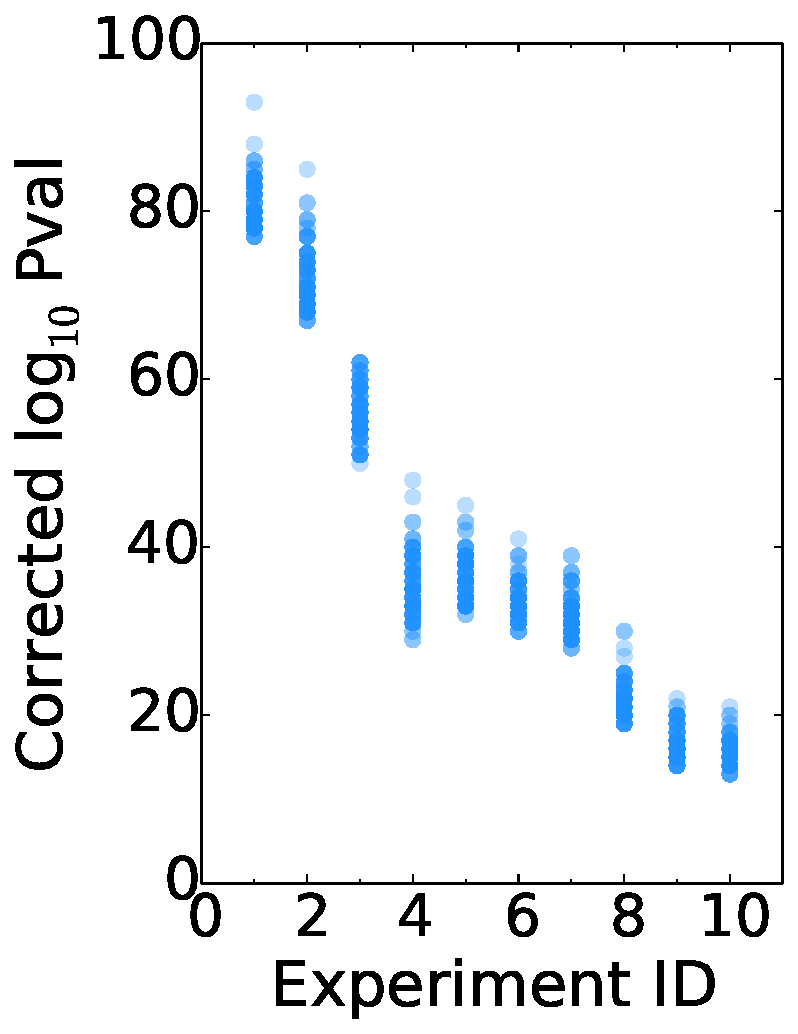
\includegraphics[width=.16\textwidth]{fig/msig_singleF.pdf}}
\subfigure[\lincs]{\label{fig:lincs_singleF}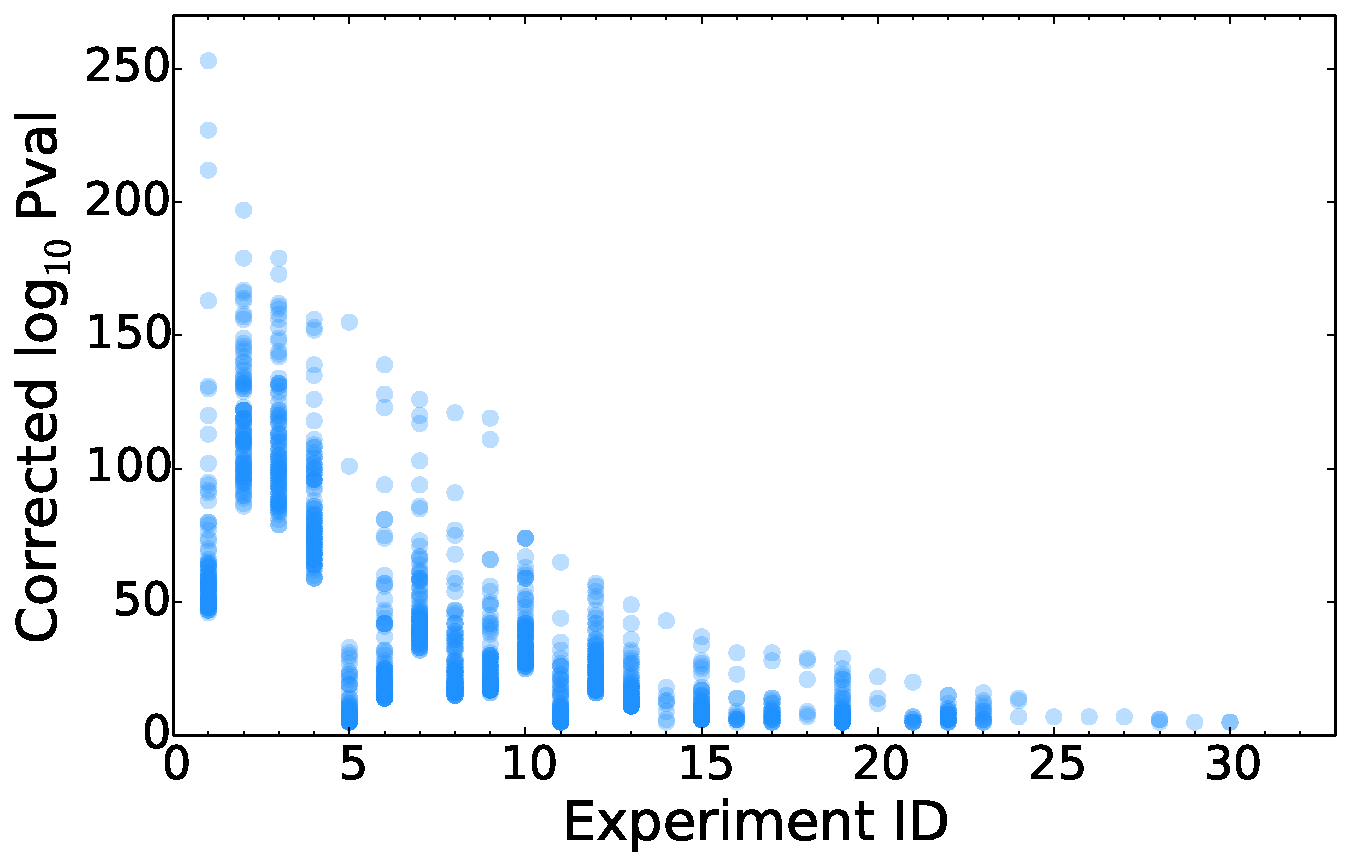
\includegraphics[width=.31\textwidth]{fig/lincs_singleF.pdf}}
\vspace{-5mm}
\caption{Top-100 Single Features' Corrected P-value Distribution}
\vspace{-5mm}
\label{fig:singleF}
\end{figure}

\begin{figure}[h]
\centering     %%% not \center
\vspace{-5mm}
\subfigure[\msig]{\label{fig:msig_FP}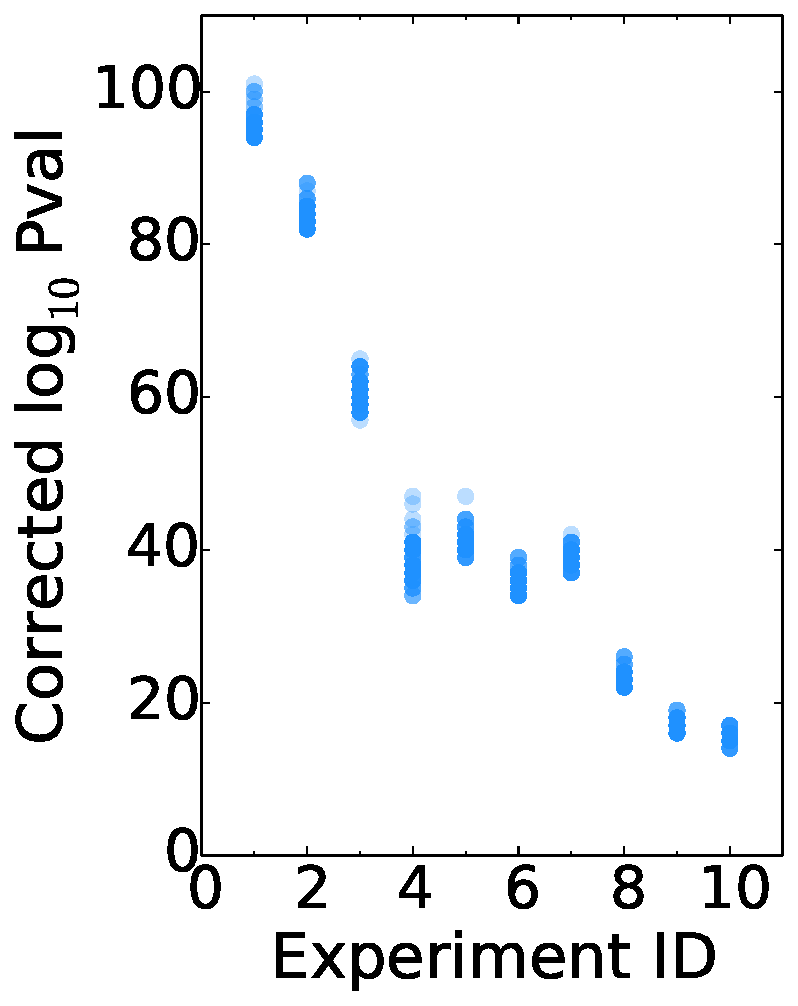
\includegraphics[width=.16\textwidth]{fig/msig_FP.pdf}}
\subfigure[\lincs]{\label{fig:lincs_FP}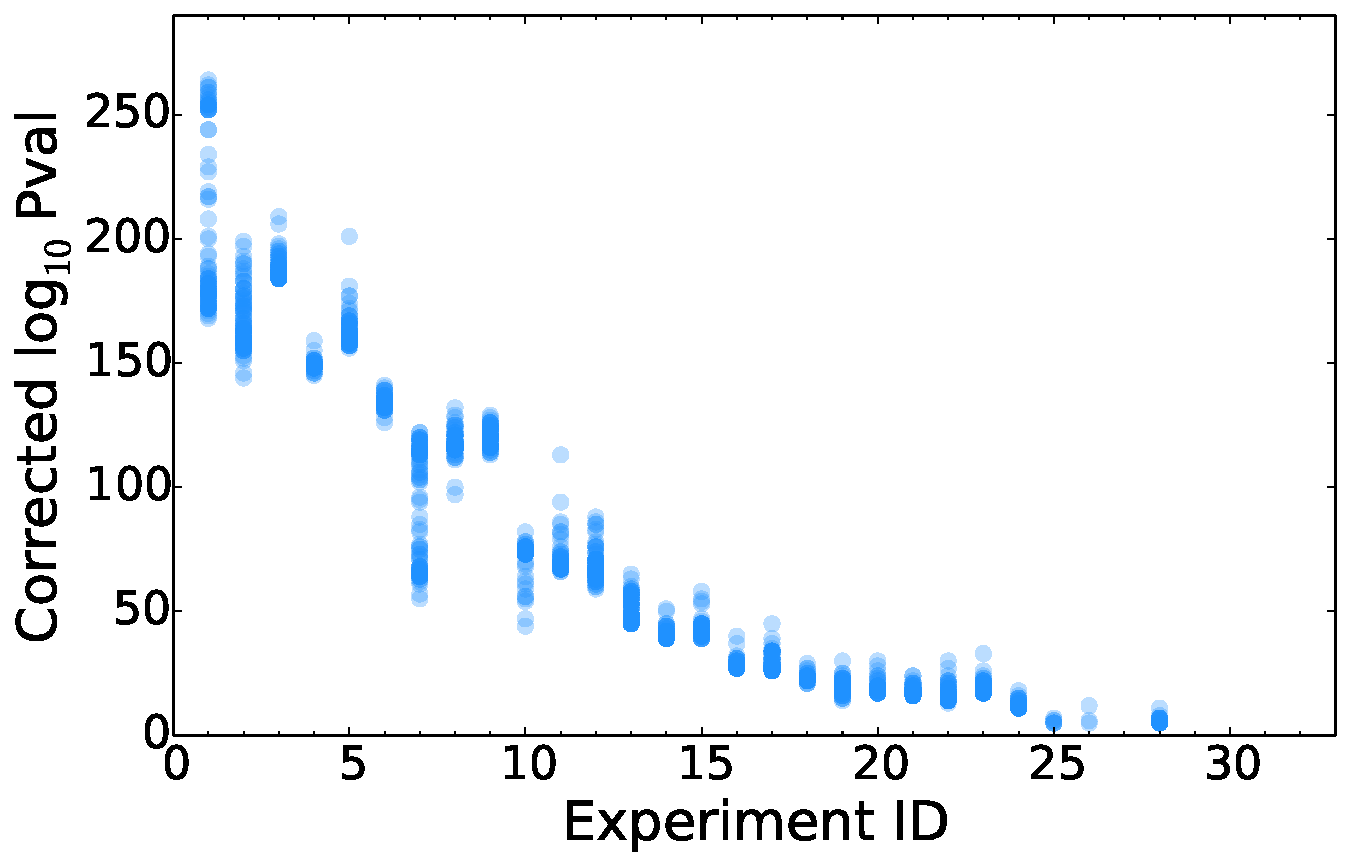
\includegraphics[width=.31\textwidth]{fig/lincs_FP.pdf}}
\vspace{-5mm}
\caption{Top-100 Feature Pairs' Corrected P-value Distribution}
\vspace{-5mm}
\label{fig:FP}
\end{figure}

\stitle{Feature Pair.} We plot the distribution of the corrected p-value for \topk feature pairs in Figure~\ref{fig:FP}. Different from single features, the corrected p-value equals $correct\_pval = pval\times m^2 \times n^2$, since there are $m^2$ possible feature pairs and $n^2$ possible separating lines. The threshold, defining a good feature pair, is also set to $10^{-5}$. We can see that 10 out of 10 experiments in \msig and 27 out of 32 experiments in \lincs have good feature pairs. Furthermore, we observe that the density distribution changes dramatically from Figure~\ref{fig:singleF} to Figure~\ref{fig:FP}. Take \lincs as an example, the upper part with small corrected p-value is very sparse in Figure~\ref{fig:singleF}, while it is much denser in Figure~\ref{fig:FP}. This indicates that the \topk feature pairs have better separability performance compared to single features. In the following, we further illustrate that feature pairs provide better and new insights compared to single features. 

\begin{figure}[h]
\centering     %%% not \center
\vspace{-3mm}
\subfigure[\msig]{\label{fig:msig_histogram_diff}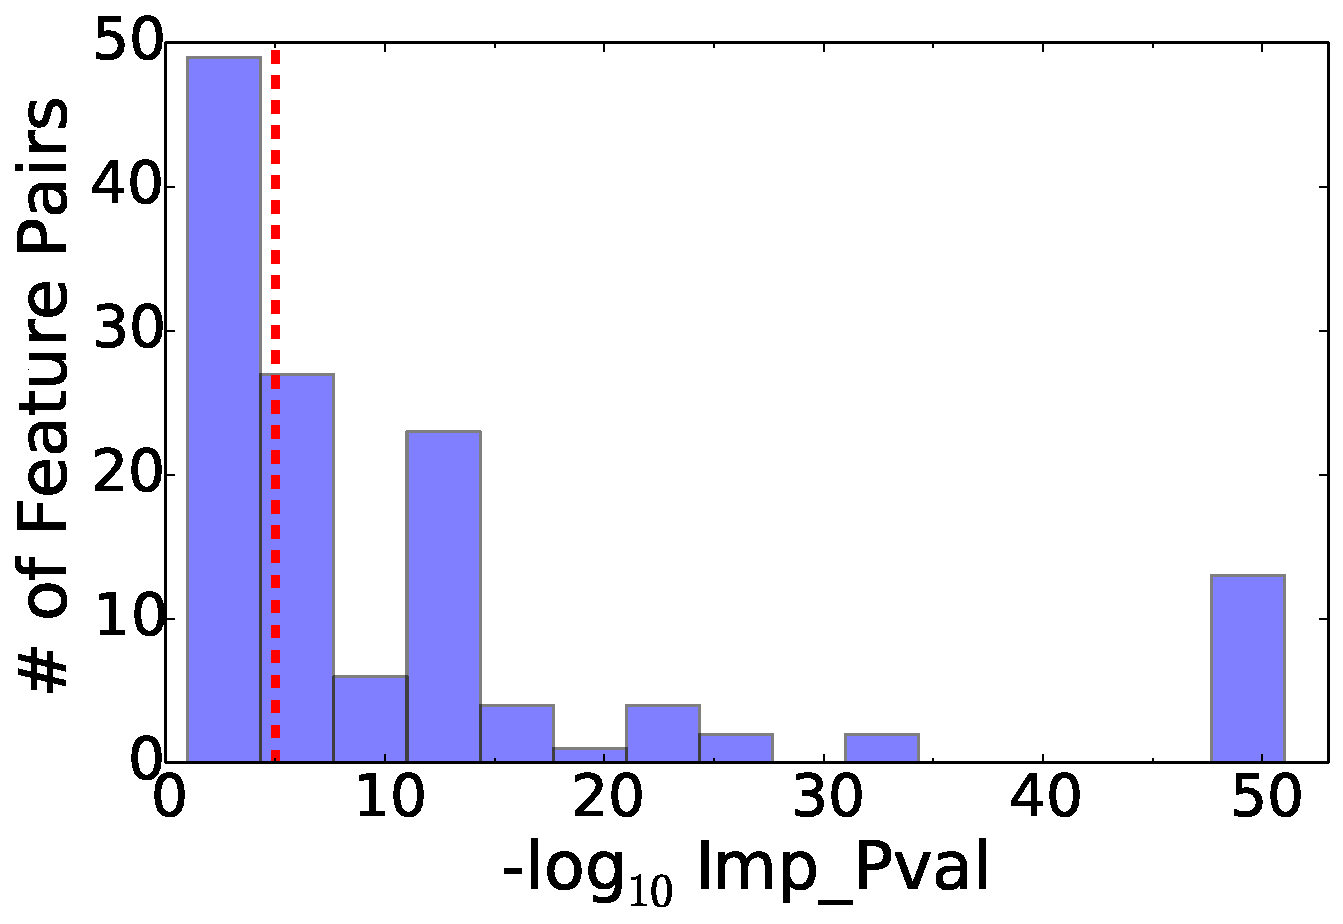
\includegraphics[width=.235\textwidth]{fig/histogram_msig_diff_pval.pdf}}
\subfigure[\lincs]{\label{fig:lincs_histogram_diff}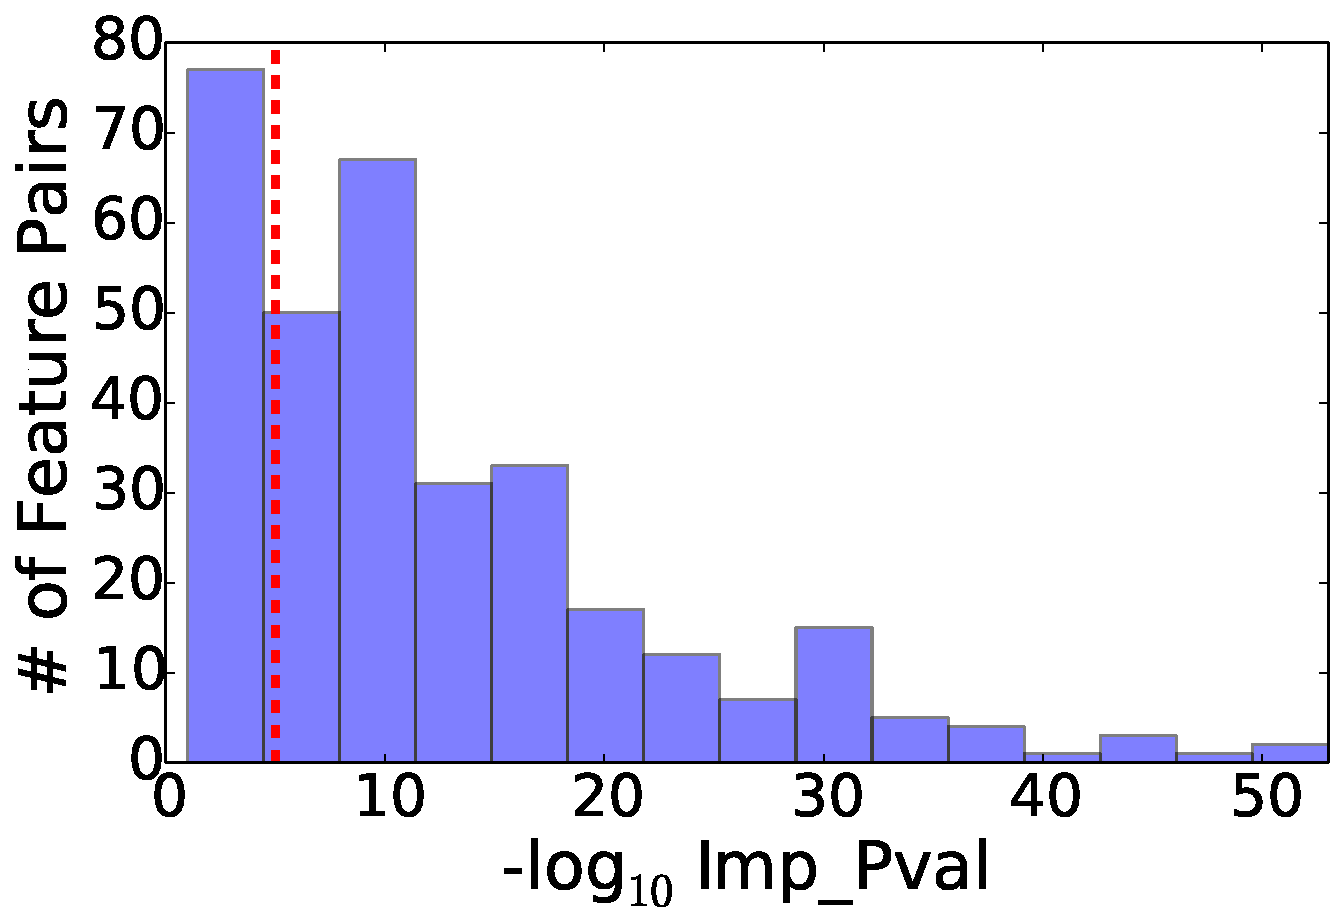
\includegraphics[width=.235\textwidth]{fig/histogram_lincs_diff_pval.pdf}}
\vspace{-5mm}
\caption{Histogram of $Imp\_Pval$ for Top-20 Feature Pairs}
\vspace{-5mm}
\label{fig:histogram_diff}
\end{figure}


\stitle{Improvement from Single Feature to Feature Pair.} We have computed the corrected p-value $correct\_pval$ for each single feature and feature pair. Now let us examine the improvement of each feature pair from its corresponding single feature in terms of p-value. For each feature pair $(f_i,f_j)$, we define the improved p-value as the ratio between the corrected p-value of $(f_i,f_j)$ and the better corrected p-value of $f_i$ or $f_j$, i.e., $Imp\_Pval = \frac{correct\_pval(f_i,f_j)}{\min(correct\_pval(f_i),correct\_pval(f_j))}$. Remember that the correction factors for single feature and feature pair are different: $mn$ vs. $m^2n^2$. In this set of experiment, we focus on top-20 feature pairs for each experiment, since users typically end up only looking at the feature pairs within top-20. In Figure~\ref{fig:histogram_diff}, we plot the histogram of $Imp\_Pval$ for 10 experiments in \msig and 32 experiments in \lincs. As shown by the red dotted line, many feature pairs have more than $10^{-5}$ times improvement from its corresponding single feature, i.e., $-\log Imp\_Pval > 5$. This shows a great improvement from single feature to feature pair in terms of p-value from Fisher's exact test, i.e., the independence probability of the real and predicted label.




% \begin{figure}[h]
% \centering     %%% not \center
% \subfigure[\msig]{\label{fig:msig_FP}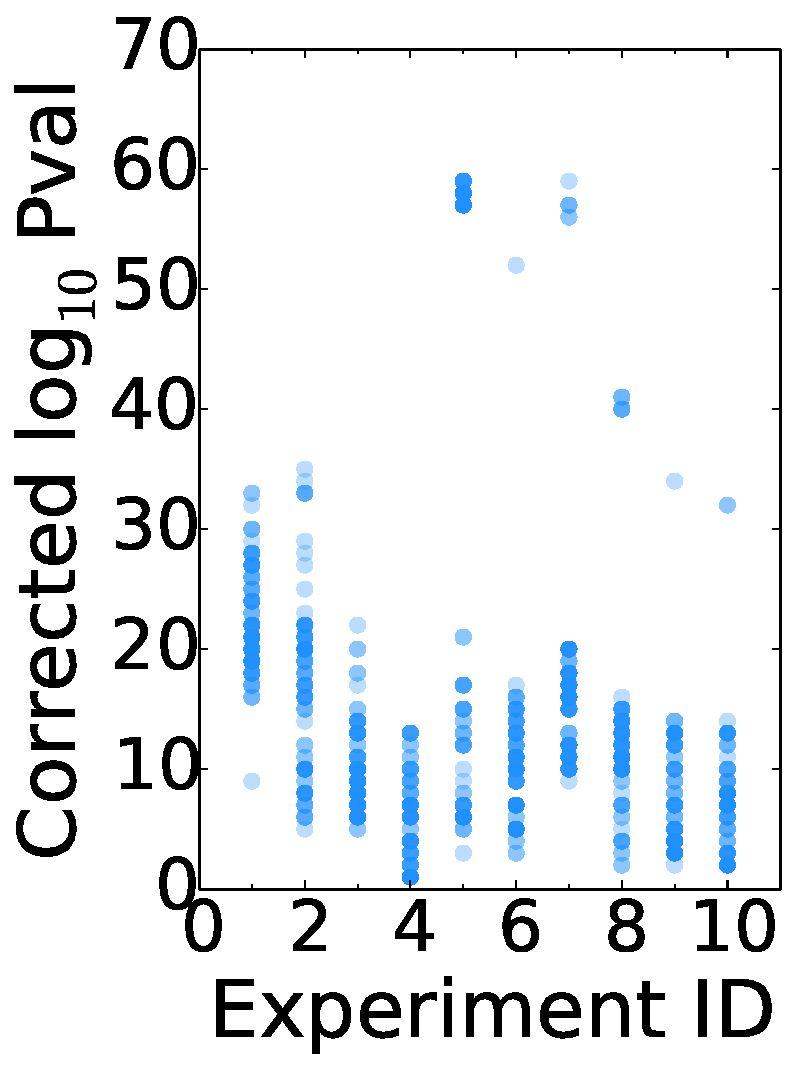
\includegraphics[width=.16\textwidth]{fig/msig_diff_pval.pdf}} # top-100
% \subfigure[\lincs]{\label{fig:lincs_FP}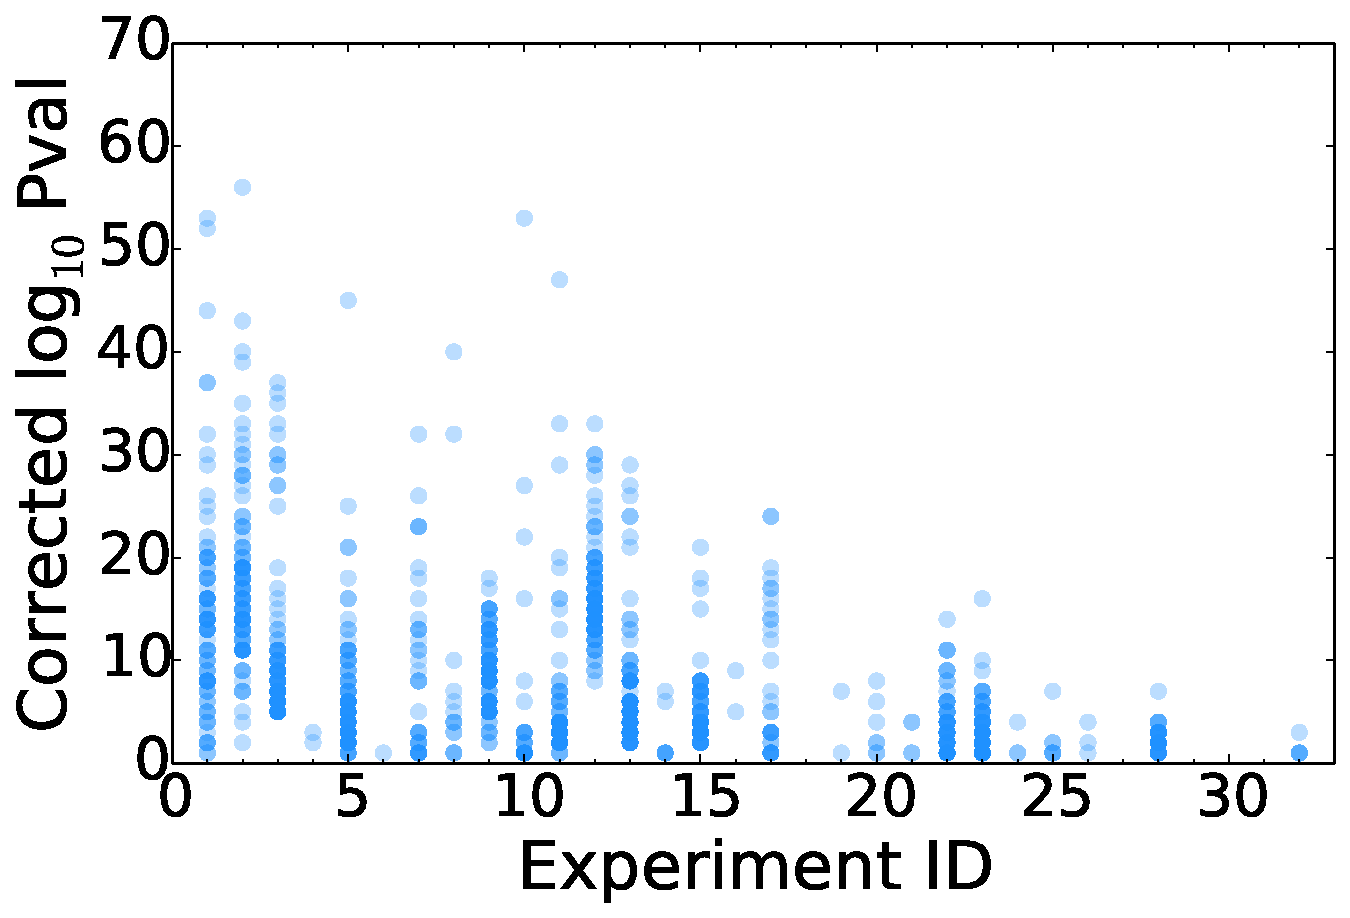
\includegraphics[width=.31\textwidth]{fig/lincs_diff_pval.pdf}}
% \caption{Top-100 Feature Pairs' Corrected P-value Distribution}
% \label{fig:FP}
% \end{figure}

\begin{figure}[h]
\vspace{-5mm}
  \centering
  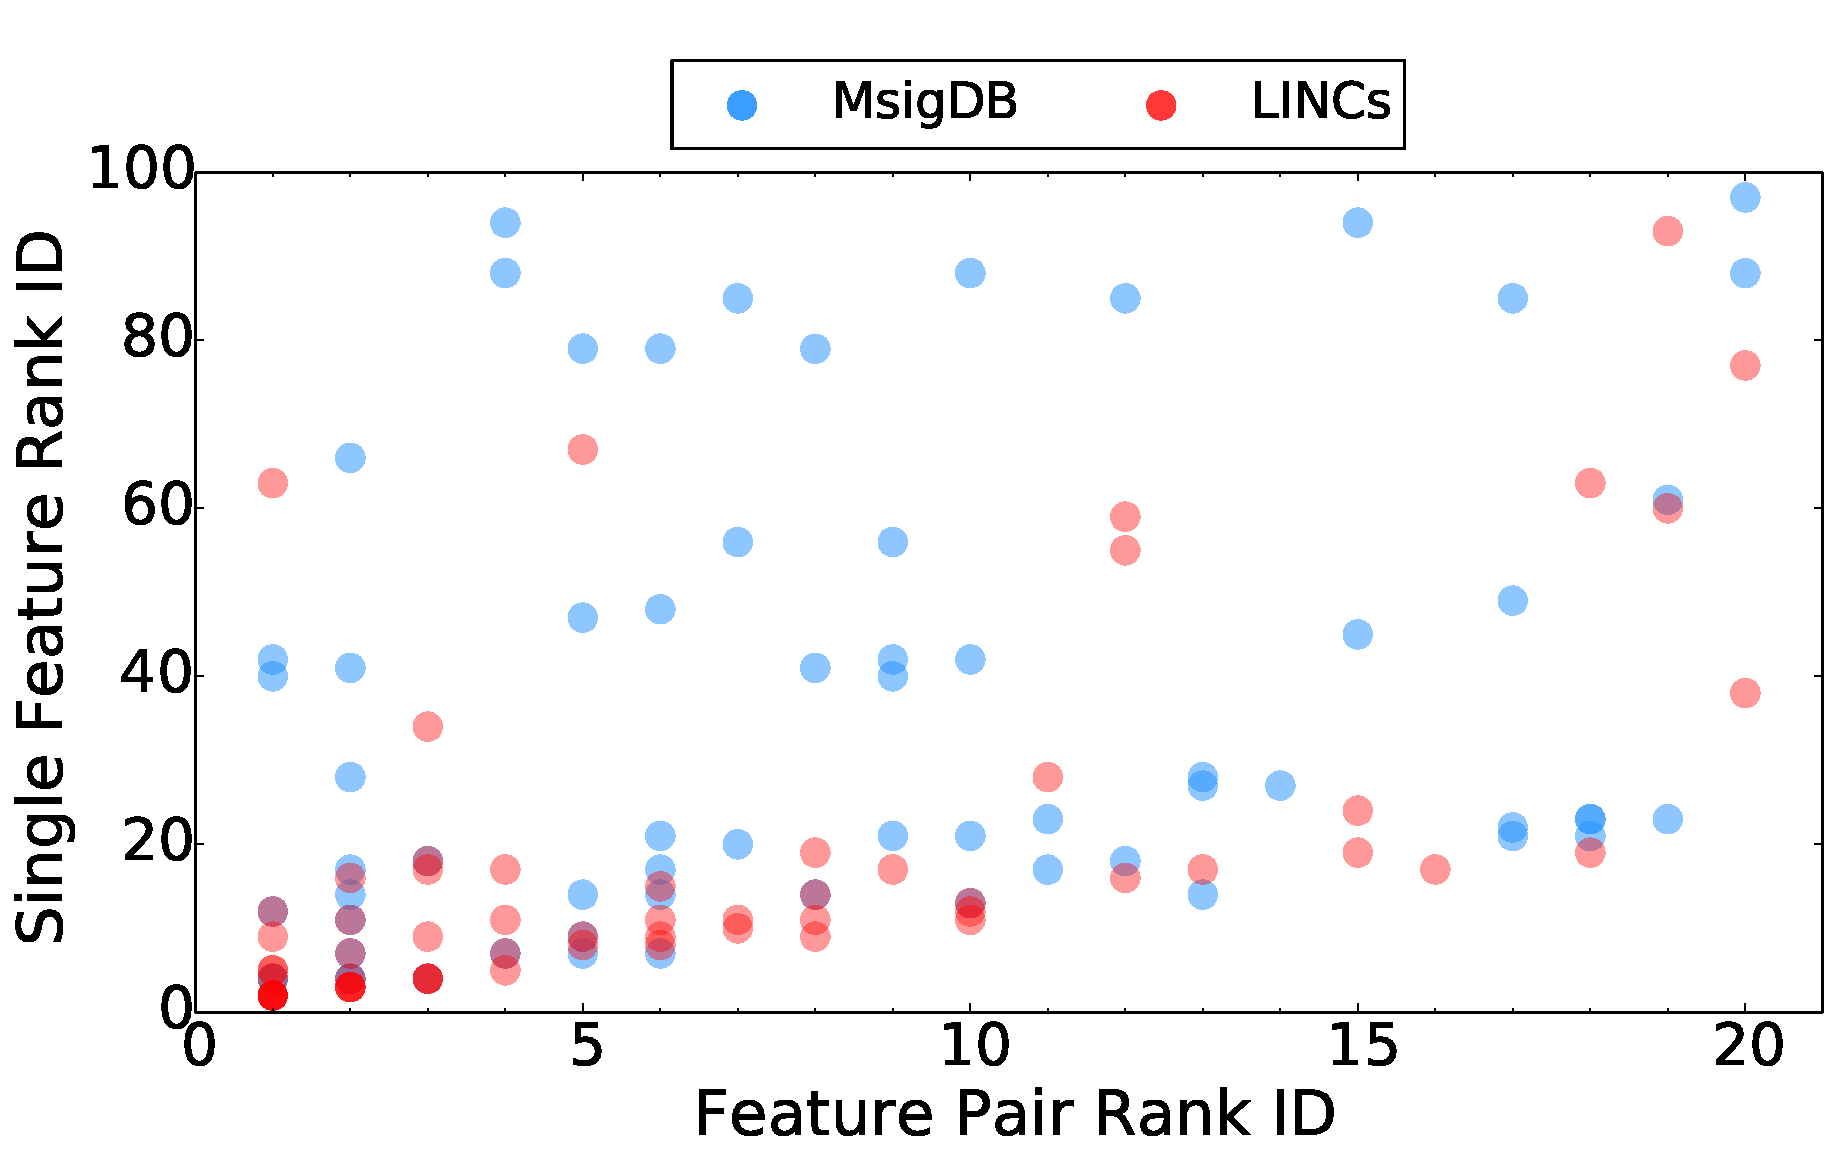
\includegraphics[width=0.8\linewidth]{fig/better_rank_20.pdf}
  \vspace{-5mm}
\caption{Feature Pair's Ranking vs. Single Feature's Ranking for Top-20 Feature Pairs}
\vspace{-5mm}
\label{fig:better_rank_20}
\end{figure} 

\stitle{New Insight from Feature Pair.} The question asked here is whether there exists some high-ranked feature pairs whose corresponding single features are poorly-ranked individually. If so, then we say the feature pair reveals new insights. Again, we focus on top-20 feature pairs, since typically users will only explore feature pairs within top-20. Given a feature pair $(f_i,f_j)$, we compare the feature pair's ranking with the better ranking of its corresponding single feature $f_i$ or $f_j$, i.e., $\min(rank(f_i),rank(f_j))$. Figure~\ref{fig:better_rank_20} illustrates the feature pairs, whose ranking is better than its individual feature's ranking. First, we observe that many high-ranked feature pairs consist of two single features that rank poorly individually than the composed feature pair, as shown by the scatterplot in Figure~\ref{fig:better_rank_20}. Furthermore, the feature pairs in the upper part of Figure~\ref{fig:better_rank_20} provide new insights that top single features fail to detect. For instance, in one experiment of \lincs, the best feature pair (the left-most red point in Figure~\ref{fig:better_rank_20}) is made up of two single features ranked outside of the top-60 individually. This feature pair can form an interesting hypothesis for further analysis or experiment. Hence, \genviz focuses on feature pairs as well as single features.



% \begin{figure}[h]
% \centering     %%% not \center
% \subfigure[\msig]{\label{fig:msig_FP}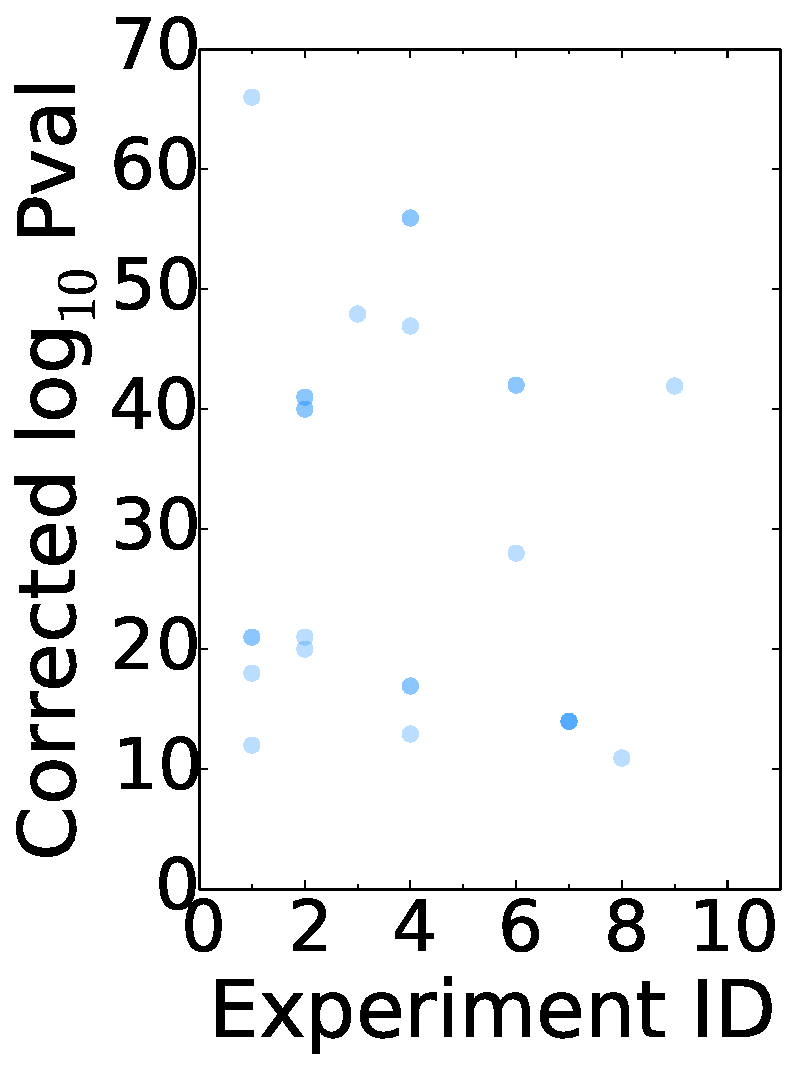
\includegraphics[width=.16\textwidth]{fig/msig_better_rank.pdf}}
% \subfigure[\lincs]{\label{fig:lincs_FP}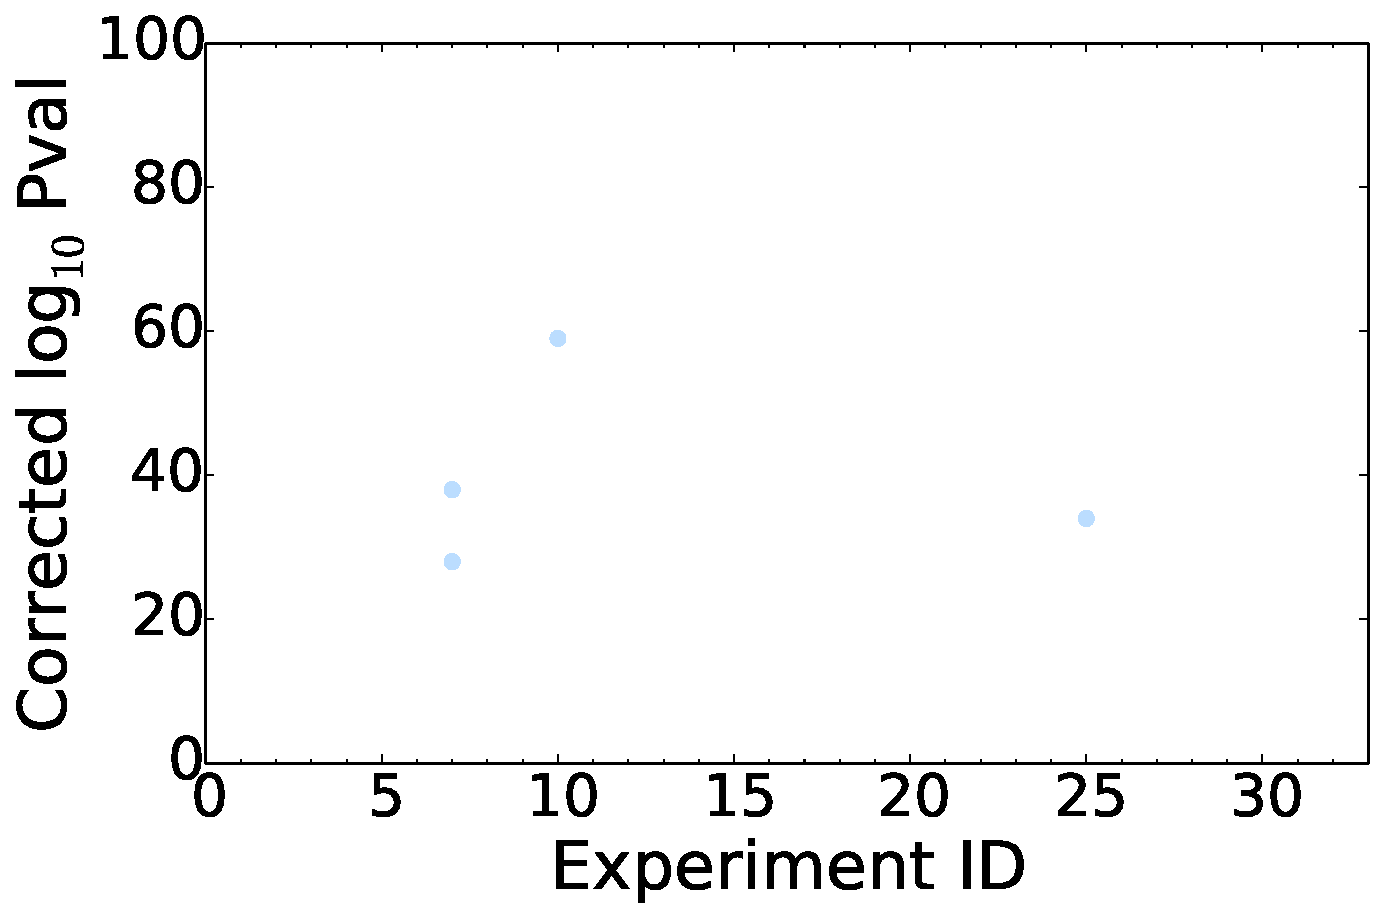
\includegraphics[width=.31\textwidth]{fig/lincs_better_rank.pdf}}
% \caption{Top-100 Feature Pairs' Corrected P-value Distribution}
% \label{fig:FP}
% \end{figure}



\begin{figure}[h]
\centering     %%% not \center
\vspace{-3mm}
\subfigure[\msig]{\label{fig:viz_msig}\includegraphics[width=.235\textwidth]{fig/ratioHist_msig_1.pdf}}
\subfigure[\lincs]{\label{fig:viz_lincs}\includegraphics[width=.235\textwidth]{fig/ratioHist_LINCS_1.pdf}}
\vspace{-5mm}
\caption{Visualization Output of \genviz}
\vspace{-5mm}
\label{fig:viz}
\end{figure}

\subsection{Output Visualization}
As discussed in Section~\ref{sec:intro}, the output of \genviz is not simply a separability score, but also a visualization to help users interpret the separability. 
In the following, we depict one sample output visualization from \msig and one from \lincs in Figure~\ref{fig:viz}. We use heatmap to illustrate the distribution of positive objects (in red) and negative objects (in blue) under the selected feature pair $(f_i,f_j)$, where $f_i$ is x-axis, $f_j$ is y-axis, and the caption is the experiment's name. For the ease of interpretation, we also add the centroids of positive and negative objects using red circle and blue circle respectively.
Now let us explain the separability in Figure~\ref{fig:viz}. For \msig, we can see that the stationary probability for negative objects is clustered around zero, while positive objects have higher stationary probability overall. For \lincs, positive objects all have one probe up and one probe down, much different from the negative objects with zero-mean Gaussian distribution.
Hence, outputting the visualization is a good way to help users better explain the separability and understand the data. 









